\chapter{R3 hardvér}
\label{kap:2}
Nasledujúca kapitola je venovaná vyhotoveniu zariadenie z pohľadu hardvéru. Hovorí o častiach, z ktorých sa zariadenie skladá, o ich parametroch, funkciách a vlastnostiach. Taktiež porovnáva poslednú verziu vyhotovenia – verzia R3, so staršími verziami zariadenia, vysvetľuje, prečo sme sa pre dané zmeny rozhodli a ako vplývajú na celkové fungovanie zariadenia. Medzi výraznejšie zmeny patrí napríklad implementácia nového snímača - gyroskopa alebo nový typ prevodového systému. Kapitola najprv vysvetľuje schému zapojenia nášho zariadenia, neskôr detailnejšie opisuje jednotlivé komponenty, z ktorých sa zariadenie skladá. Tiež opisuje výber vhodného telesa pre náš systém, implementáciu nového spôsobu prevodu rotačného pohybu zo servomotora na trubičku a tvorbu nových 3D prvkov. V závere sa nachádza zoznam všetkých komponentov a súčiastok, z ktorých sa zariadenie skladá a hovorí o jeho výslednej cene. 

\section{Schéma zapojenia}
\label{kap:2.1}

Schéma zapojenia nášho zariadenia prešla od poslednej verzie niekoľkými zmenami. Celkovo by sa dala rozdeliť na 2 oddelené schémy, ktoré sú vzájomne prepojené pomocou FFC (flat flexible cable) káblu. Oddelenie schém je potrebné z dôvodu, že senzory na snímanie polohy guličky v trubičke a pootočenia ramena musia byť umiestnené na trubičke. Z toho vyplýva že schéma celého našeho zariadenia musí byť oddelená aby mohli byť vytvorené 2 PCB dosky, ktoré v celku tvoria jednu schému. Prvou je časť zariadenia nachádzajúca sa na hlavnej PCB doske (obr. \ref{OBRAZOK 2.1.1} ), ktorú priamo zapájame do Arduina. Obsahuje servomotor (a) , ktorý je napájaný 5 V a je pripojený k arduinu () prostredníctvom pinu 9, cez ktorý prijíma od arduina PWM signál, potrebný na riadenie polohy otočenia jeho hriadeľa. K servomotoru je pripojený aj kondenzátor (g) a dióda (j). Úlohou kondenzátora je vyhladiť prechodové javy, ktoré by mohli ovplyvniť napájanie serva a dióda slúži ako ochrana pred poškodením obvodov spätným EMF – elektromotorickým napätím. Potenciometer (c) je napájaný napätím 3,3 V a k arduinu je pripojený pomocou analógového pinu A0, ktorý slúži na získavanie hodnôt, ktoré neskôr transformujeme do formy, v ktorej môžu byť použité ako referenčná hodnota pre riadenie polohy.  Zmenou v schéme zapojenia oproti poslednej verzii je implementácia lineárneho regulátora napätia – LDO (b), potrebného pre zmenu hladiny napätia pre napájanie snímačov. Je pripojený k zdroju napätia o veľkosti 5V, ktorého hladinu upravuje a už zmenenú posiela na konektor pre FFC kábel (d). Ten slúži na prepojenie jednotlivých schém do jedného celku. Je pripojený k pinom SCL a SDA na arduine, ktoré slúžia na sprostredkovanie I2C komunkácie. Ku LDO sú paralelne pripojené 2 kondenzátory (h) (i), ktoré sú na základe informácii z datasheetu [] potrebné pre fungovanie LDO a ich parametre sú pre daný lineárny regulátor napätia zadané. 
\begin{figure}[]
	\centering
	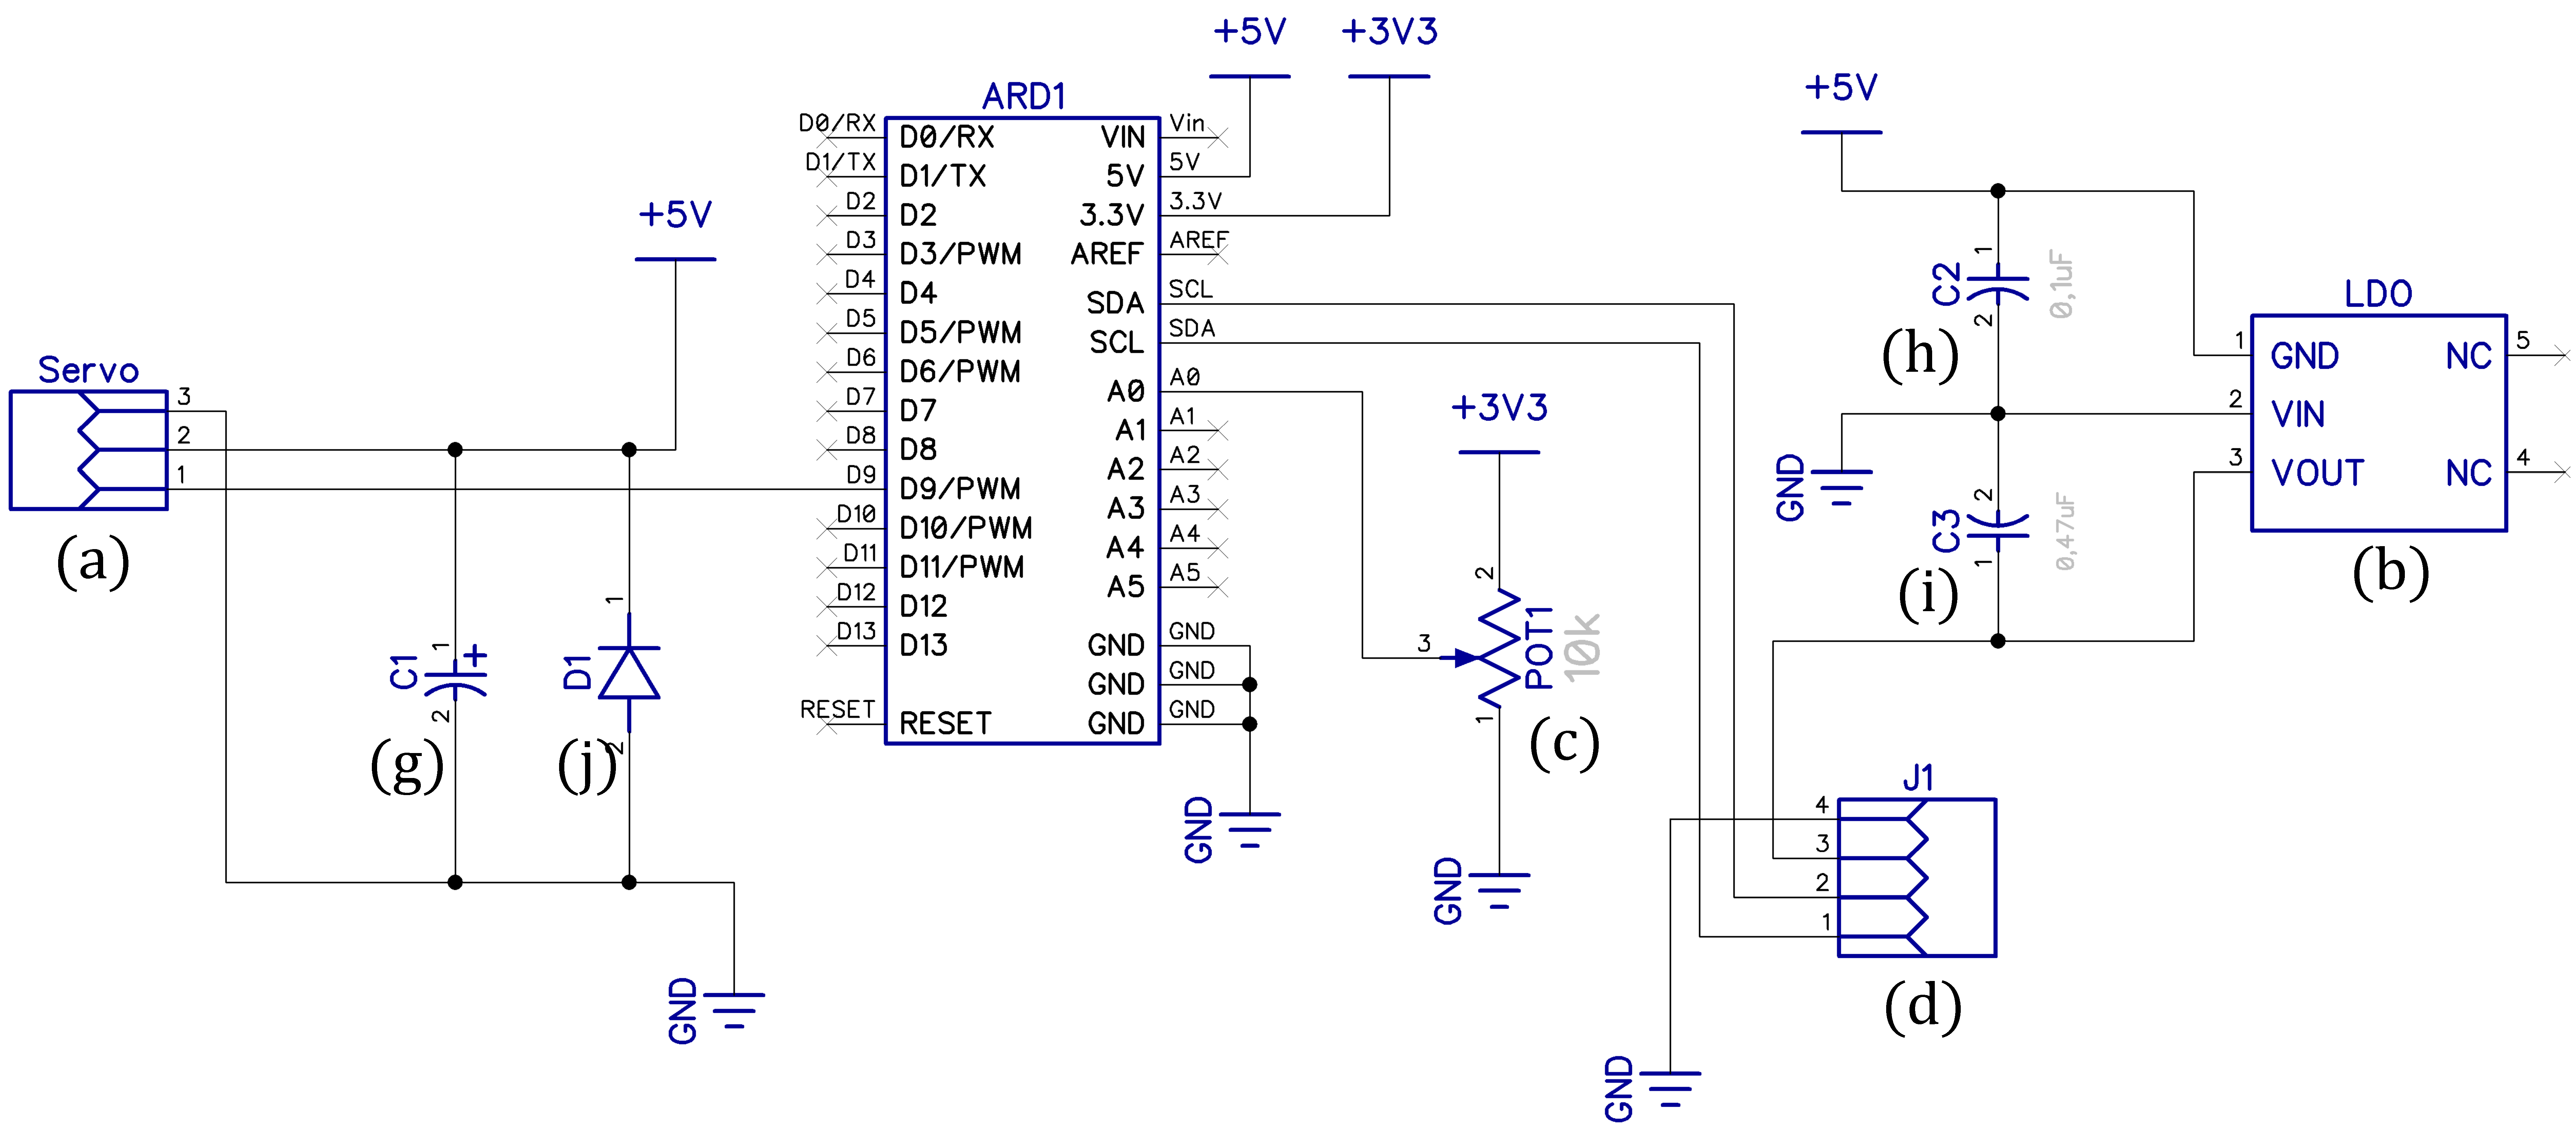
\includegraphics[width=150mm]{obr/BoBshield.eps}
	\caption{Schéma hlavnej PCB dosky}\label{OBRAZOK 2.1.1} 
\end{figure} 

Druhá časť schémy (obr. \ref{OBRAZOK 2.1.2} ) je nami navrhnutá breakout doska, nachádzajúca sa na konci trubičky a obsahuje naše snímače. Snímač polohy – VL6180X (e) je pripojený ku konektoru (d), ktorý mu poskytuje napájacie napätie a taktiež sprostredkováva I2C komunikáciu medzi snímačom a arduinom. Gyroskop – MPU-6050 (f) je rovnako ako snímač polohy napájaný cez konektor (d) a taktiež je paralelne pripojený k 2 kondenzátorom (k) (l). Ich potreba vyplýva z informácii poskytnutých v datasheete [], kde je uvedený správny spôsob zapojenia snímača aj parametre kondenzátorov. Rezistory (m) (n) slúžia ako pull up rezistory pri I2C komunikácii snímačov s arduinom. 
\begin{figure}[]
	\centering
	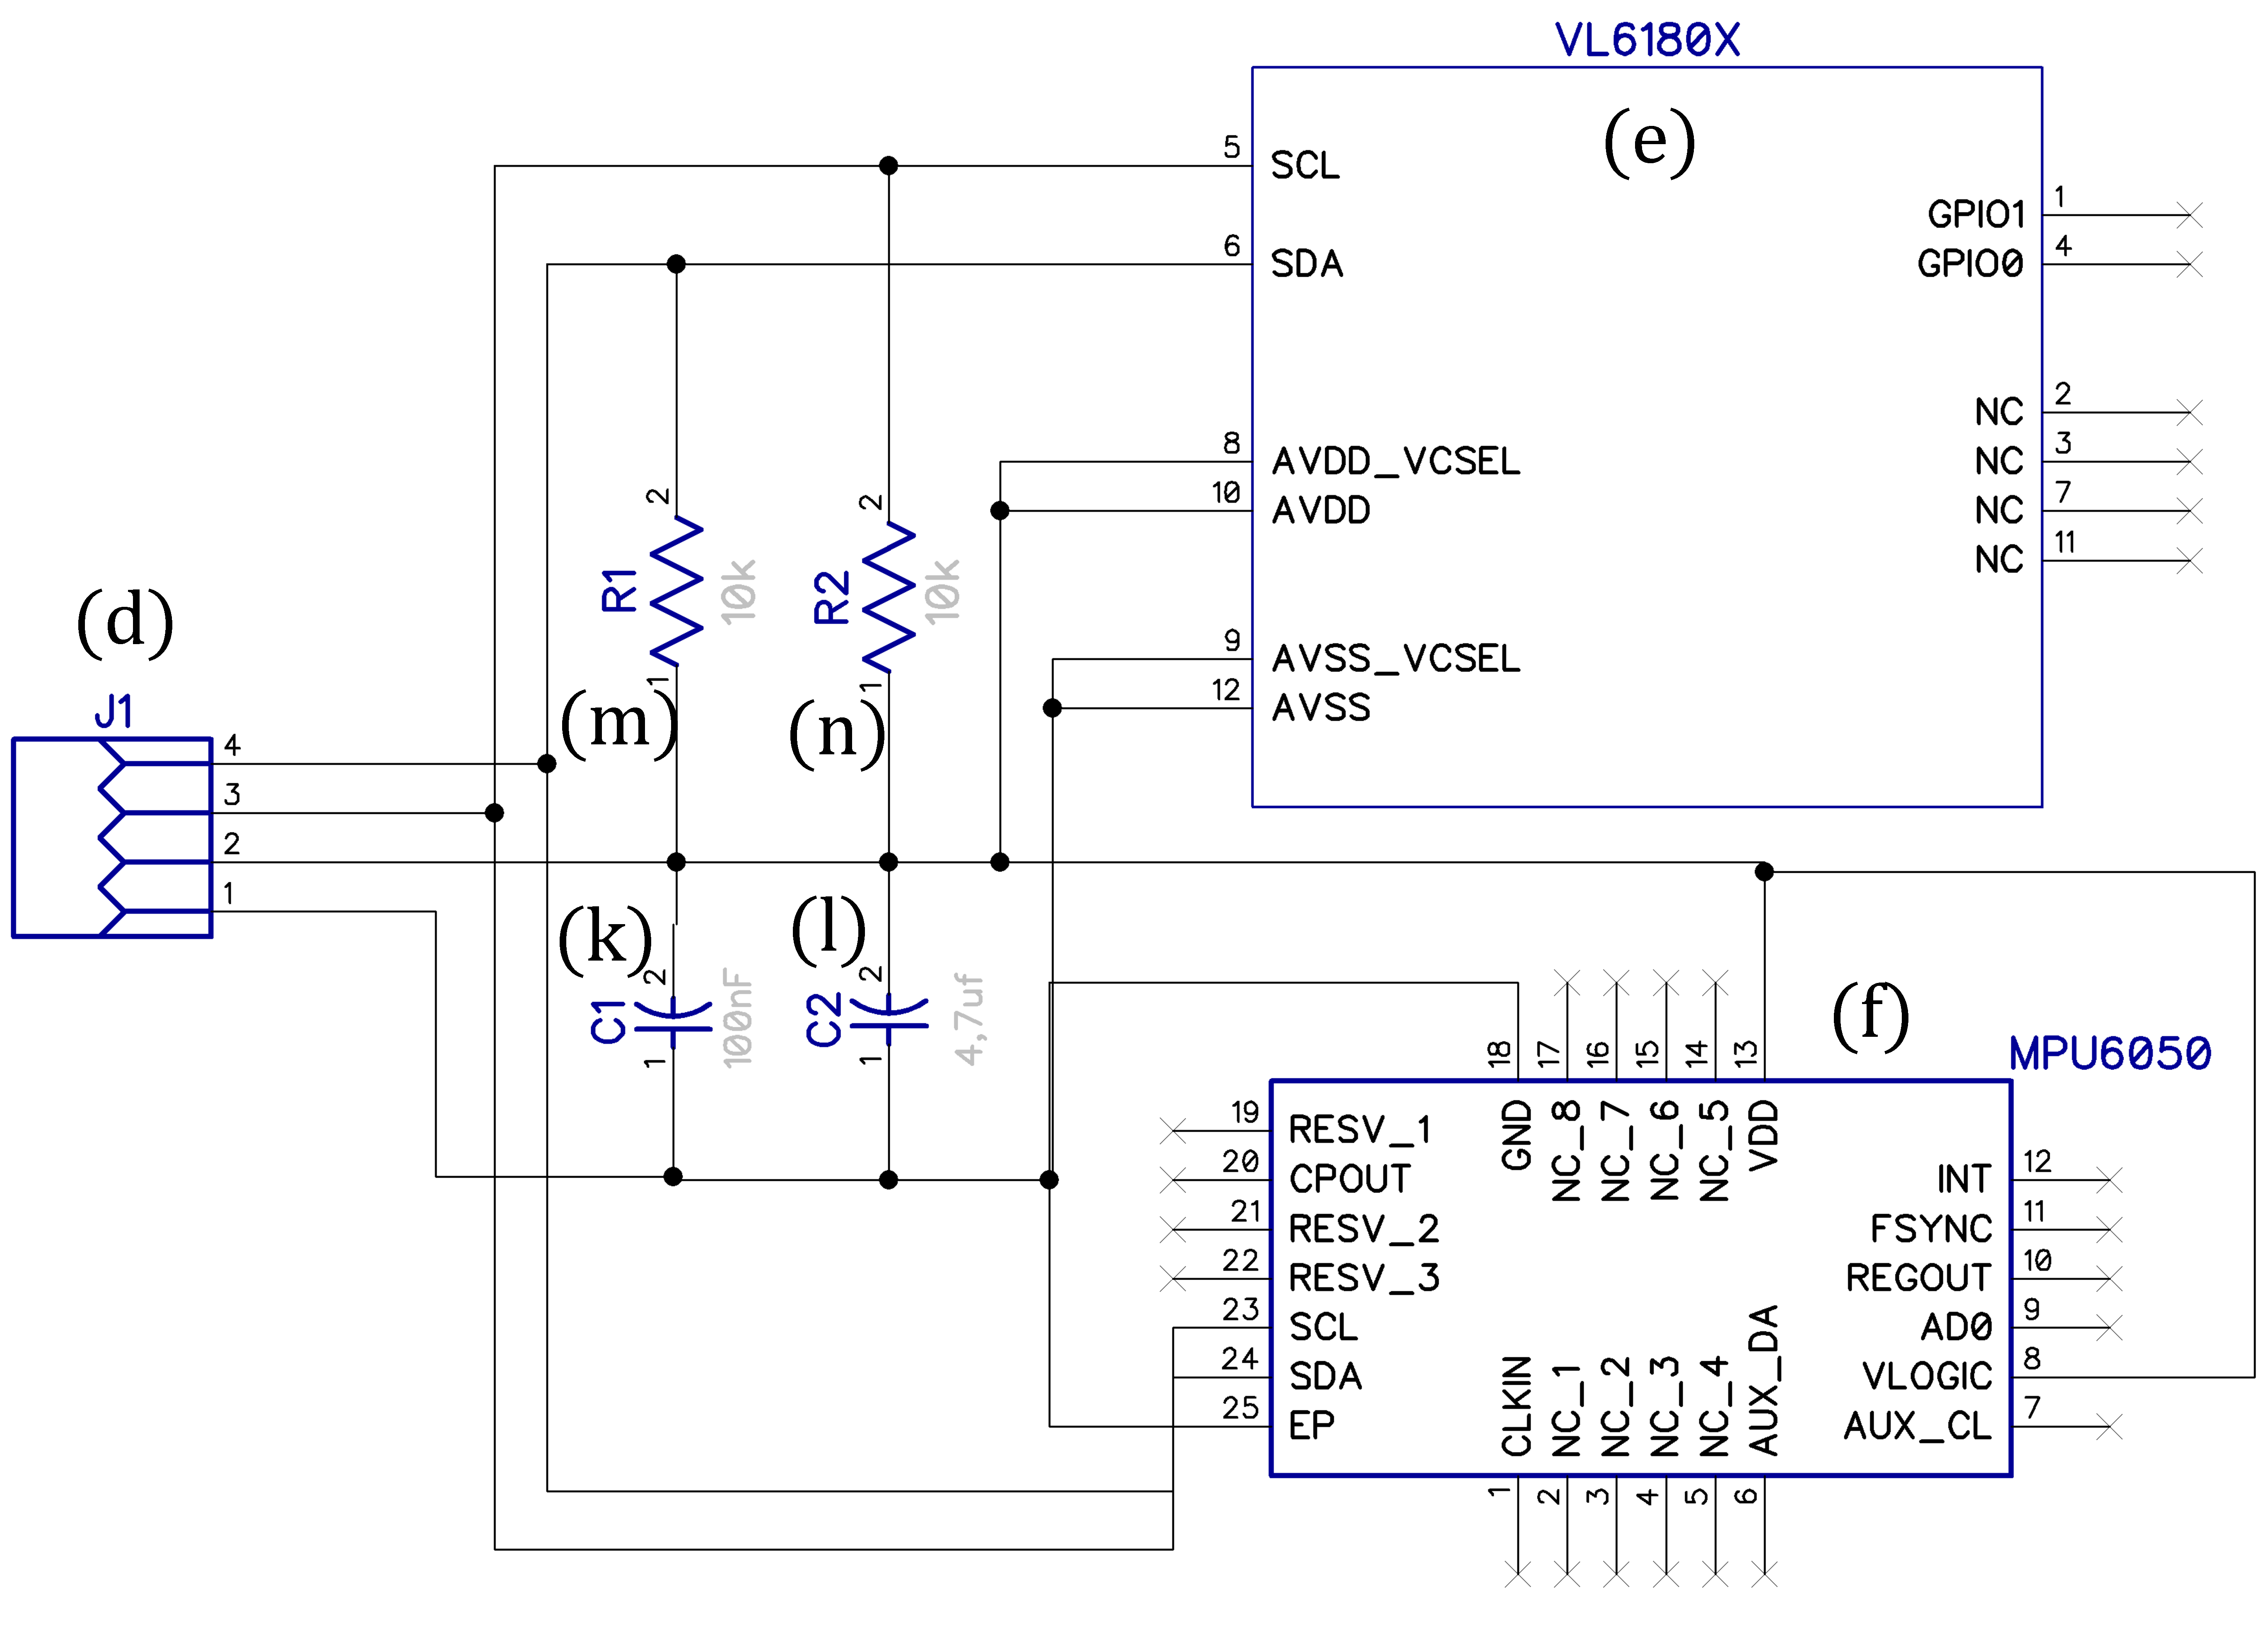
\includegraphics[width=100mm]{obr/senzors.eps}
	\caption{Schéma PCB dosky so snímačmi}\label{OBRAZOK 2.1.2} 
\end{figure} 

Obe schémy boli navrhnuté vo voľne dostupnom software DIPTrace. 

 
% Obrázky schém + opis 
% Obrázky PCB dosiek + opis
Po návrhu schémy zapojenia jednotlivých dosiek sme pristúpili k ich fyzickému návrhu. Pri tvorbe hlavnej PCB dosky sme museli pracovať s tvarom dosky shieldu pre arduino, na ktorú sme sa snažili vhodne umiestniť jednotlivé komponenty a konektory.  Na hlavnej doske (obr.\ref{OBRAZOK 2.1.3} a obr.\ref{OBRAZOK 2.1.4}) sa okrem elektronických komponentov budú nachádzať aj 3D prvky zariadenia, preto treba počítať aj s ich umiestnením a vhodne zvoliť diery určené pre montáž týchto prvkov k doske (o). Na doske sa teda nachádza spoj pre pripojenie servomotora (a) a  potenciometer pre získavanie referenčnej hodnoty (c), ktorých umiestnenie sme nechali v rovnakej polohe ako pri pôvodnej verzii dosky. Ich poloha je vzhľadom na umiestnenie 3D prvkov ideálna, keďže konektor servomotora sa nachádza v dostatočnej blízkosti pre jeho pripojenie a zároveň nemusíme použiť zbytočne dlhý kábel. Potenciometer sa tiež vzhľadom ku 3D modelu nachádza vo vhodnej pozícii, keďže jeho umiestnenie je ovplyvnené práve potrebou možnosti pohybovať s bežcom počas chodu zariadenia. Preto je potrebné aby nedochádzalo k vzájomnej interakcii medzi pohyblivými časťami zariadenia a rukou užívateľa pri nastavovaní referenčnej hodnoty. Umiestnenie kondenzátora (g) a diódy (i) je tiež podľa pôvodnej verzii. Umiestnenie konektoru pre FFC káble (d) sme zvolili tak, aby sa po montáži kompletného zariadenia nachádzal pod trubičkou a tak nedochádzalo k jeho zahnutiu a spĺňalo to aj estetickú funkciu. Na základe jeho pozície došlo k umiestneniu spoja pre LDO (b), keďže jeho úlohou je zmena hladiny napätia do rozsahu napájacích napätí snímačov, nachádza sa medzi konektorom FFC kábla (d) a zdrojom napätia z arduina.  Kondenzátory (h) (i), na základe informácií z datasheetu [] potrebné pre fungovanie LDO, sú umiestnené v jeho tesnej blízkosti ako je odporúčané.

Pri návrhu PCB dosky určenej pre snímače (obr. \ref{OBRAZOK 2.1.5}), sme neboli obmedzení žiadnym konkrétnym tvarom dosky, preto bolo našim cieľom dosiahnuť rozloženie jednotlivých komponentov optimálnym spôsobom aby sme dosiahli čo najmenšie rozmery. Na hornej časti dosky môžeme nájsť plošný spoj pre umiestnenie snímača MPU-6050 (f), konektor pre pripojenie FFC kábla (d) a jednotlivé komponenty (g) (h) (i) (j), ktorých implementácia vyplýva zo schémy zapojenia jednotlivých snímačov, ktorú je možné nájsť v datasheetoch []. Na spodnej strane PCB dosky sa nachádza spoj pre umiestnenie snímača VL6180X (e). Umiestnenie snímača na spodnej strane je z dôvodu aby smeroval do vnútra trubičky, v ktorej sa nachádza gulička. Po umiestnení PCB dosky do držiaka na konci trubičky, snímač VL6180X smeruje do vnútra trubičky a z naopak FFC kábel smeruje von z trubičky, čo poskytuje jeho jednoduchú montáž. 

\begin{figure}[p]
	\centering
	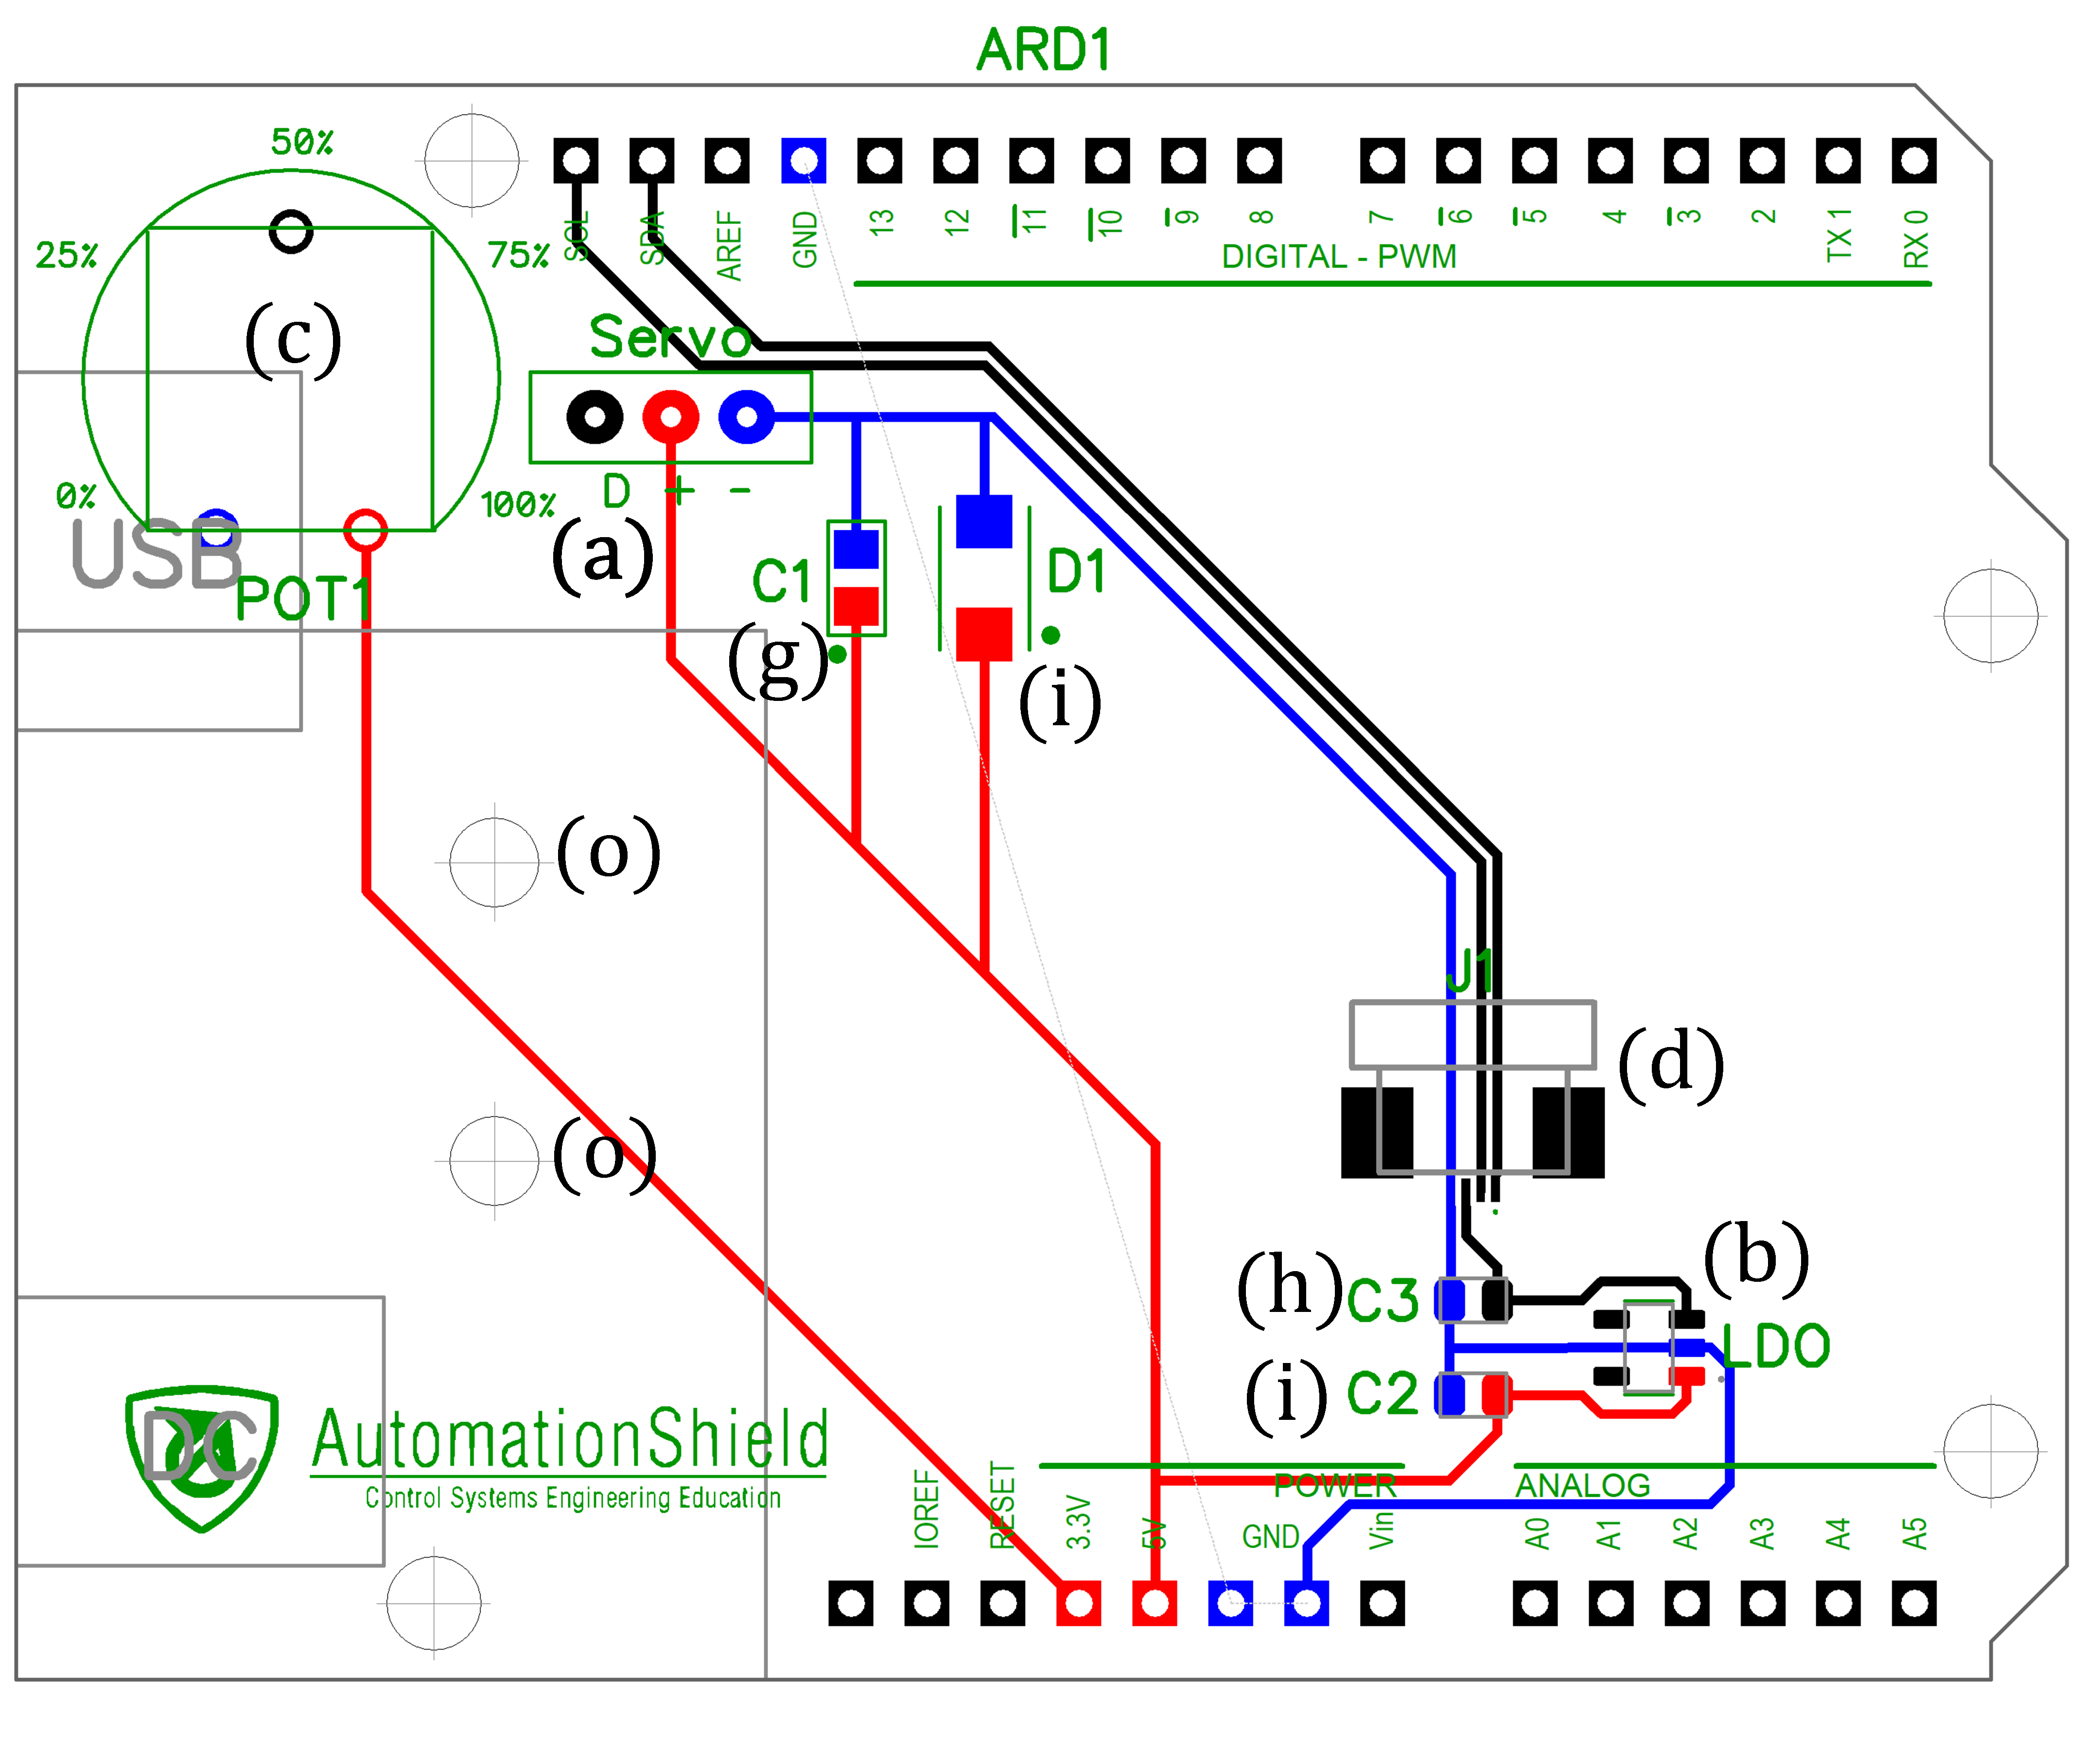
\includegraphics[width=125mm]{obr/PCBBOBup.eps}
	\caption{PCB doska - pohľad z hora }\label{OBRAZOK 2.1.3} 
\end{figure}  
 
 \begin{figure}[p]
 	\centering
 	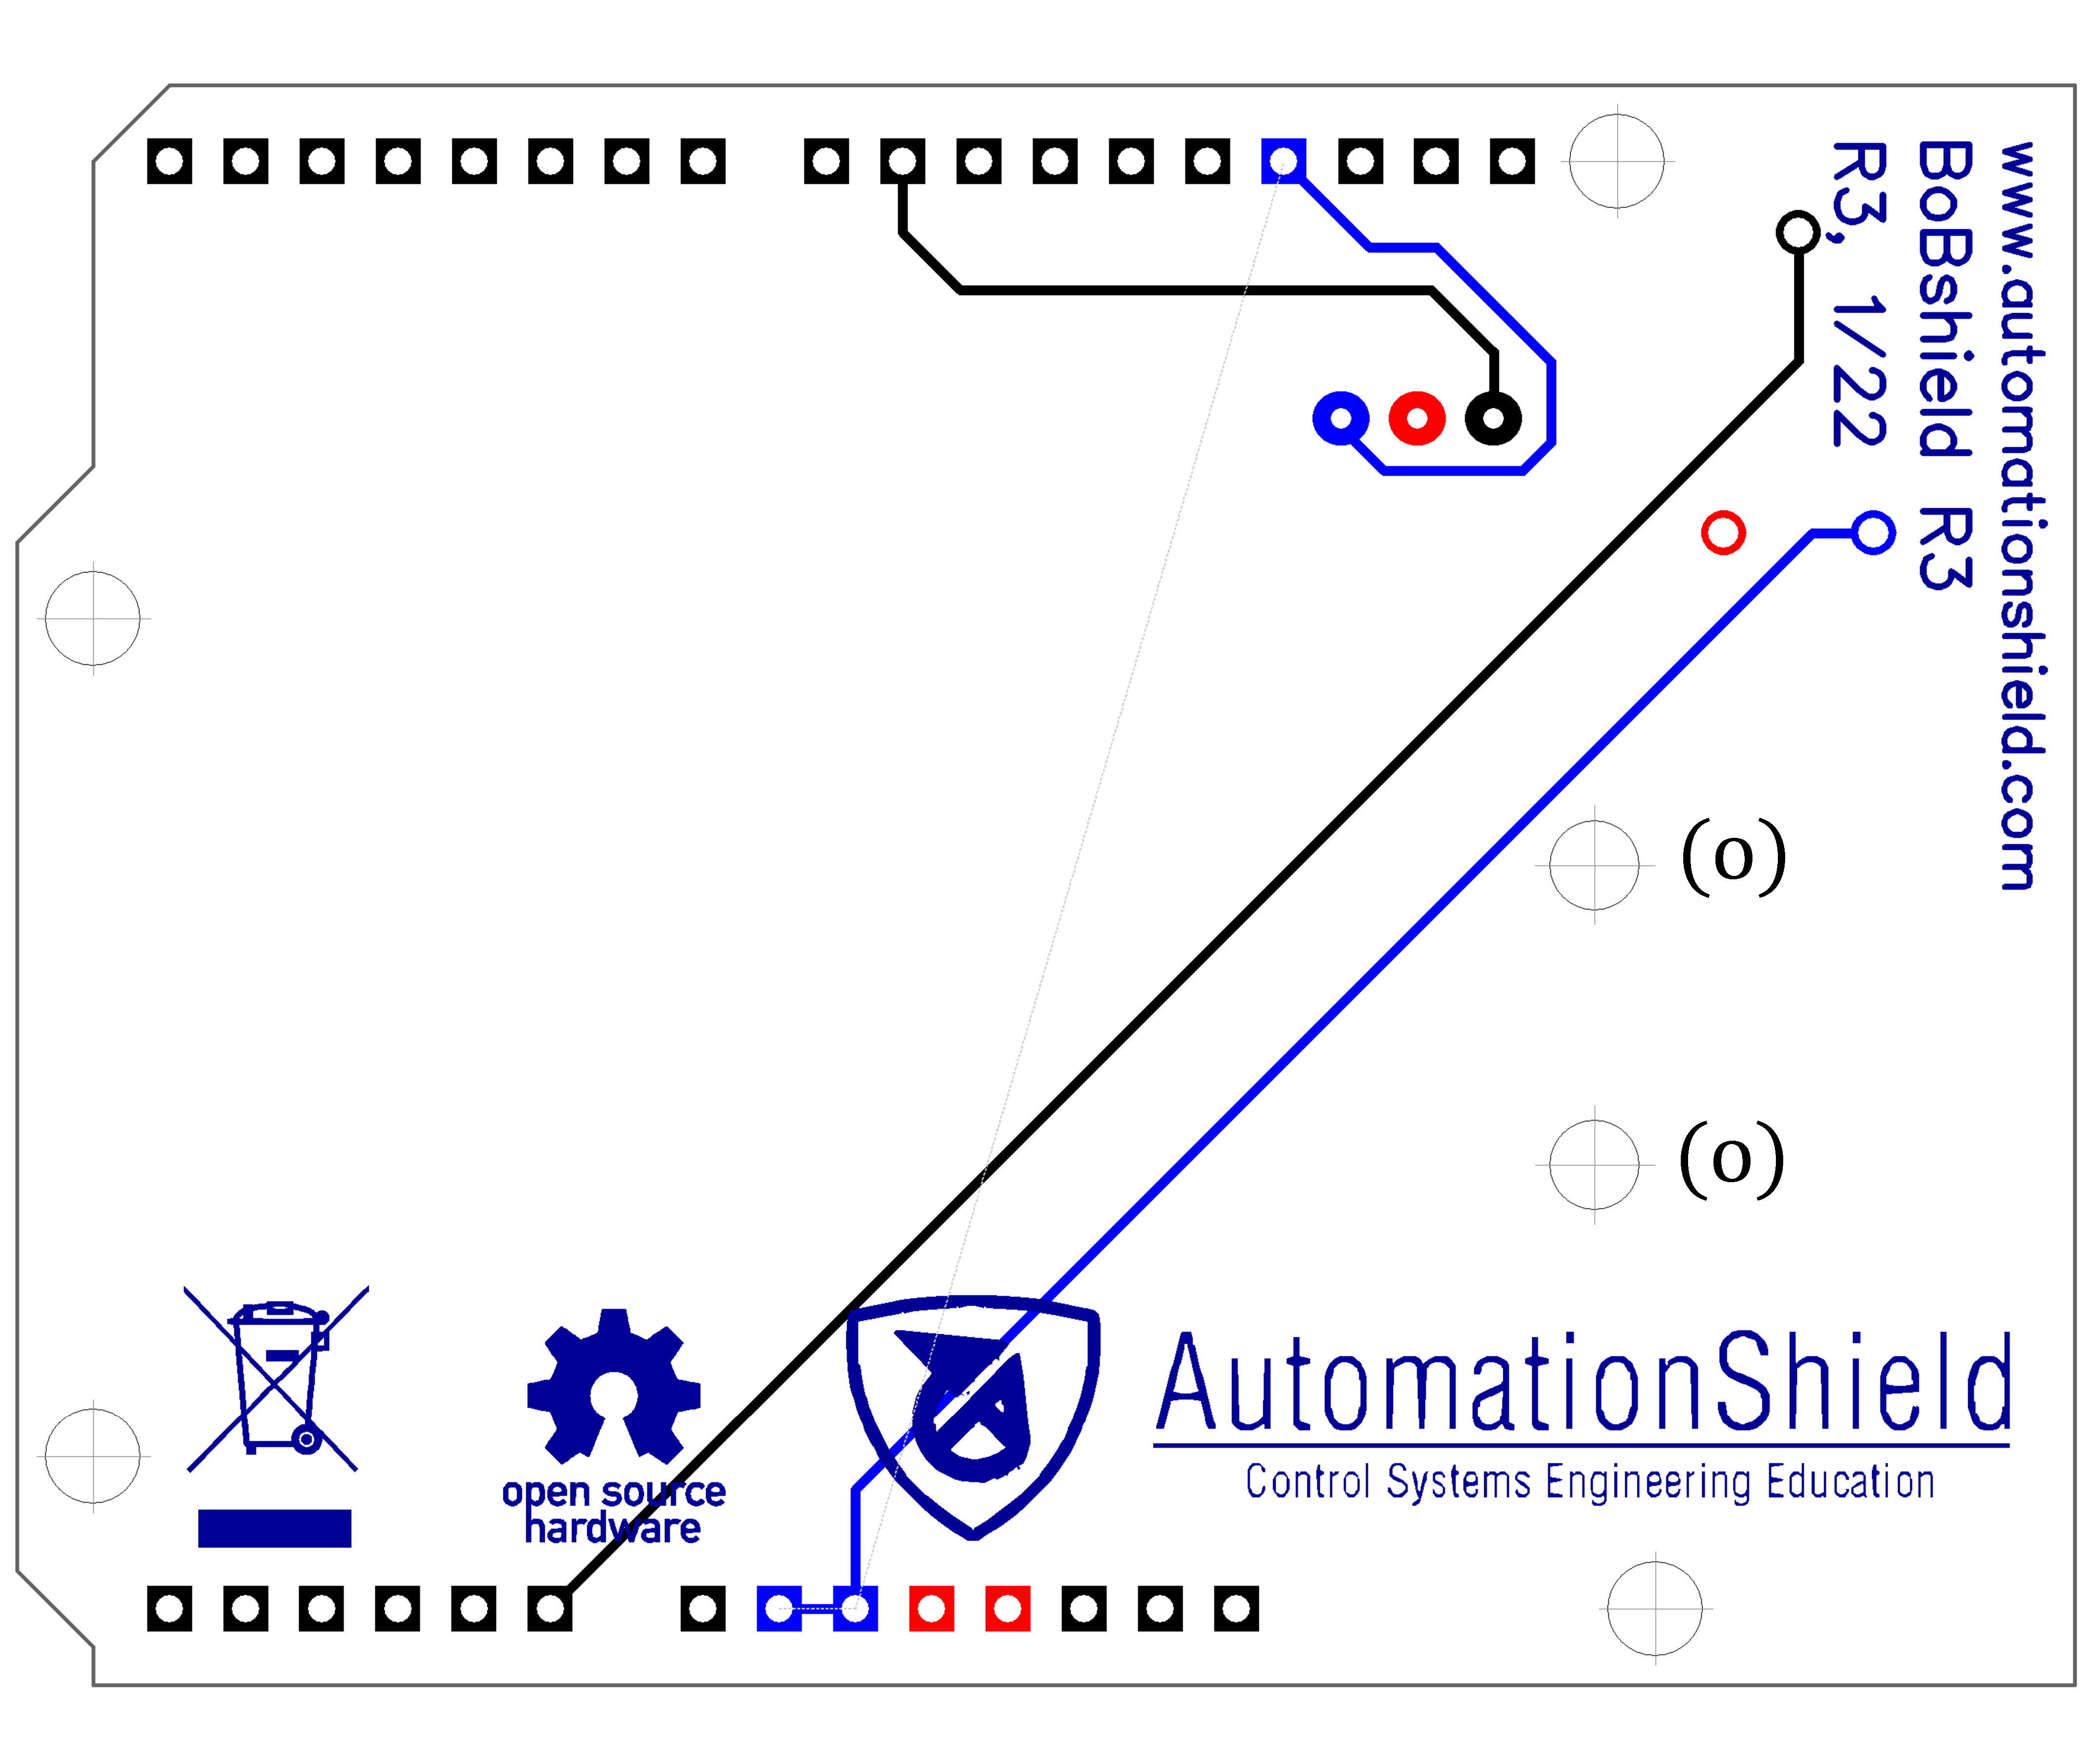
\includegraphics[width=125mm]{obr/PCBBOBbottom.eps}
 	\caption{PCB doska - pohľad z dola}\label{OBRAZOK 2.1.4} 
 \end{figure} 

 \begin{figure}[h!]
	\centering
	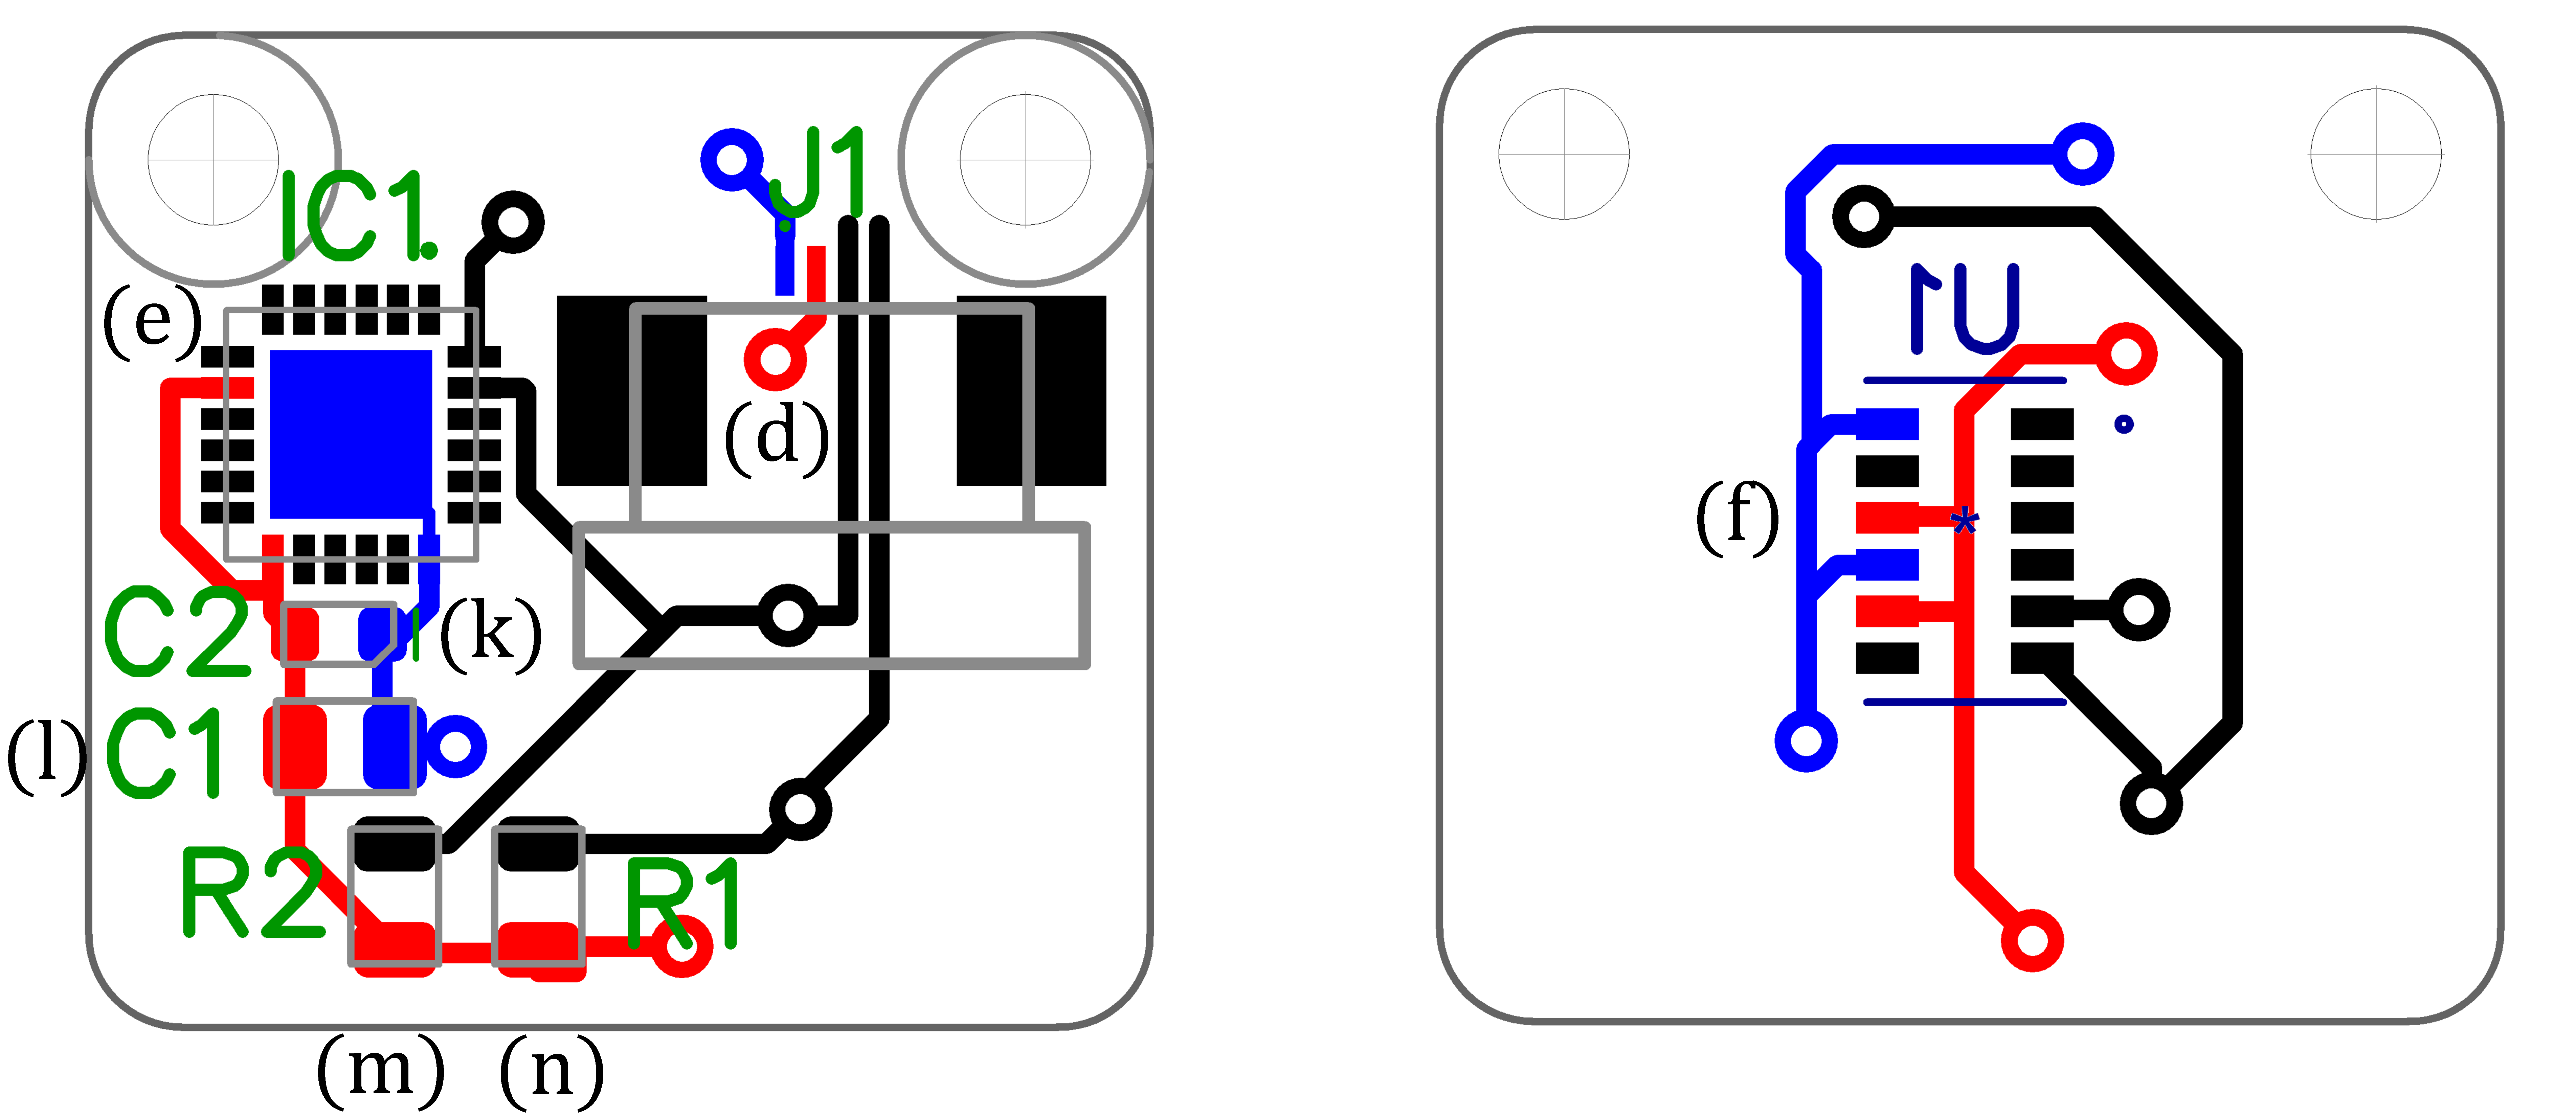
\includegraphics[width=125mm]{obr/PCBsnimace.eps}
	\caption{PCB doska pre snímače}\label{OBRAZOK 2.1.5} 
\end{figure} 
\section{Komponenty}
\label{kap:2.2}

Nasledujúca podkapitola detailnejšie opisuje vlastnosti komponentov, s ktorými sme sa už stretli pri schéme zapojenia. Hovorí o ich parametroch, funkciách, ktoré v zariadení zastrešujú a tiež opisuje proces ich výberu a dôvod prečo sme si pre naše zariadenie zvolili práve tieto komponenty. 

Pre riadenie a regulovanie akéhokoľvek systému je potrebné mať vstup do systému, ktorým nastavujeme zásah do systému. O túto časť riadiacej slučky sa starajú aktuátory. Výstup zo systému zase prezentujú hodnoty, ktoré získavame pomocou snímačov a na ich základe môžeme vyhodnocovať aktuálny stav systému.


V našom zariadení sa o jednotlivé funkcie starajú nasledujúce komponenty:
\begin{itemize}
    \item snímače – Tof snímač vzdialenosti, Gyroskop
	\item aktuátory – Servo motor 
\end{itemize}


\subsection{Servo}
\label{kap:2.2.1}
Servomotor patrí spolu so snímačmi ku komponentom, ktorých vlastnosti výrazne vplývajú na kvalitu riadenia systému. V našom systéme plní funkciu aktuátora, teda sa stará o akčný zásah do systému a tak ovplyvňuje náklon trubičky a následne pohyb guličky, ktorej polohu riadime. Na základe dôležitosti tohto komponentu sme sa rozhodli pre analýzu ponúkaných možností na trhu a ich následné porovnanie so servomotorom v pôvodnej verzii. Vo verzii zariadenia R2 bol použitý analógový servomotor  s kovovými prevodmi MG-90. Ide o veľmi rozšírený servomotor bežne sa nachádzajúci v začiatočníckych arduino kitoch, určených pre domáce projekty. Z parametrov môžeme vidieť, že spĺňa požiadavku na malé rozmery, taktiež podľa rozsahu pracovného napätie odpadá potreba jeho úpravy, a servo môže byť napájané priamo z arduina. Vďaka kovovým prevodom je jeho životnosť vyššia a dosahuje aj  lepšie presnosti oproti plastovým verziám. Čím ale servo najviac vyniká oproti iným typom a verziám je jeho nízka cena, ktorá sa pohybuje okolo 4 eur.  

Parametre:
\begin{itemize}
	\item Hmotnosť: 12 g
	\item 	Rozmery: 22.3 x 11.8 x 26.3 mm 
	\item 	Krútiaci moment: 1,8 kg (4,8 V)
	\item   Rýchlosť: 0,12 sekundy / 60 ° (4,8 V)
	\item	Prevádzkové napätie: 4.8V - 6.0V 
	\item 	Typ: Analógové
	\item	prevody: Kovové
	\item 	cena: 6 eur
\end{itemize}

Zmenu, ktorú sme teda zvažovali bolo zvoliť namiesto analógového servomotora digitálny. Ide o dilemu, s ktorou sa pri výbere servomotora stretáme veľmi často. Každý typ má svoje výhody a nevýhody no najväčším rozdielovým parametrom, od ktorého závisí výber typu serva je frekven-cia PWM signálu, s ktorým dané servo pracuje. Zároveň od toho závisia aj ostatné výhody a nevýhody, no podstata je ukrytá práve za týmto faktorom.

Princíp fungovania servomotorov je založený na prijímaní napäťového signálu , ktorý prichádya v podobe PWM (pulse width modulation – impulzová šírková modulácia) signálu. PWM signál posiela motoru elektrický impulz rôznej šírky, na základe ktorej sa otočí hriadeľ do polohy, ktorú požadu-jeme. Analógové servomotory pracujú so signálom o frekvencii 50 Hz, čo znamená že perióda jed-ného cyklu je 0,02 s, čo sa môže zdať ako dostatočne malý čas no pri riadení systému, tak dynamic-kého ako je ten náš, ide o pomerne veľký časový interval. Pri digitálnych servách dosahuje PWM signál výrazne vyššie frekvencie – pohybujeme sa v stovkách hertzov. Ak si zoberieme PWM signál o frekvencii 500 Hz, perióda jedného cyklu je 0,002 s, čo je 10 krát viac cyklov za rovnaký čas ako pri analógovom servomotore. To má za následok zníženie času kedy do serva nie je posiela-ný žiadny elektrický signál. Graficky znázornený rozdiel medzi dĺžkami cyklov PWM signálu pre digitálne a analógové servomotory, môžeme vidieť na obrázku \ref{OBRAZOK 2.1.1}. Zvýšením frekvencii teda digitálne servá dosahujú oveľa rýchlejšie reak-cie na zmeny požadovanej polohy, lepšie rozlíšenie a väčší krútiaci moment. Na druhú stranu však s väčšou frekvenciou prichádza aj väčšia spotreba energie,  vyššia cena a hluk pri prevádzke.
 
 \begin{figure}[]
 	\centering
 	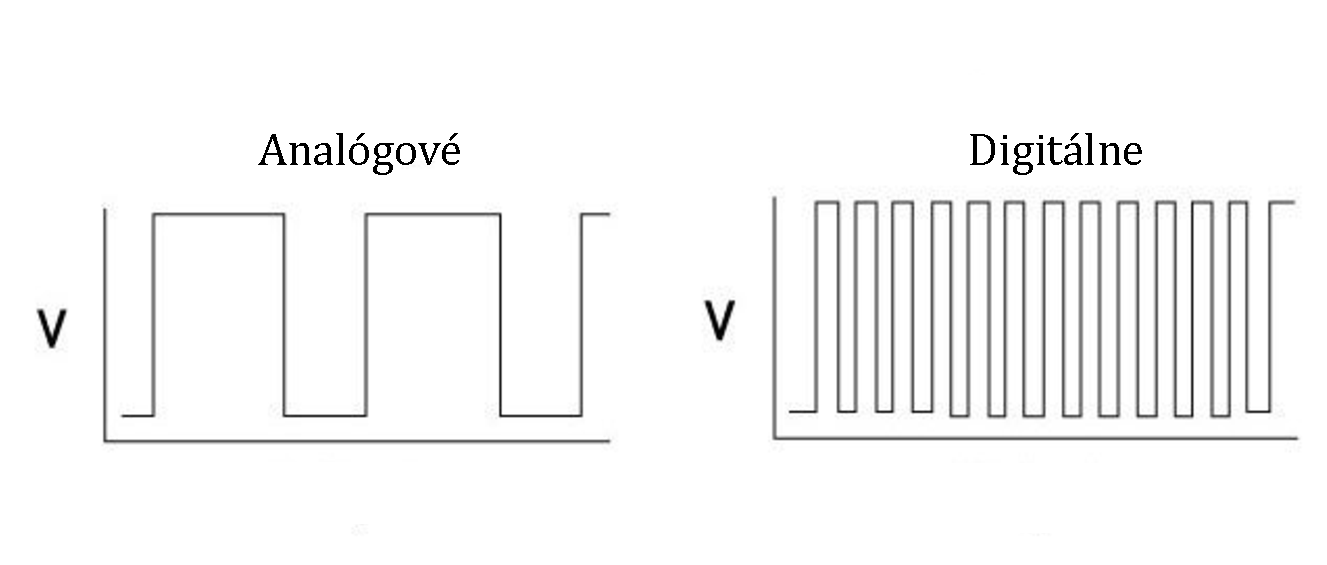
\includegraphics[width=160mm]{obr/PWMsignal.eps}
 	\caption{Dĺžka cyklu PWM signálu pre analógové a digitálne servo}\label{OBRAZOK 2.2.1} 
 \end{figure} 
 
My sme sa rozhodli pre zmenu z analógového na digitálne, z dôvodu potreby zrýchlenia reakcie aktuátora na zmenu polohy guličky a tiež lepšieho rozlíšenia pulzu. Za servomotor sme si preto zvo-lili SH-0253, digitálne servo značky SAVOX. Parametrami je veľmi podobný pôvodnému servomoto-ru MG-90. 

Parametre:
\begin{itemize}
	\item Hmotnosť: 13,6 g
	\item 	Rozmery: 23,8 x 12 x 25,4 mm 
	\item 	Krútiaci moment: 1,8 kg (4,8 V) – 2,2 (6 V)
	\item   Rýchlosť: 0,12 s/60 ° (4,8 V) – 0,9 s/60 ° (6 V)
	\item	Prevádzkové napätie: 4.8V - 6.0V 
	\item 	Typ: Digitálne
	\item	prevody: Kovové
	\item 	cena: 16 eur
\end{itemize}


\subsection{ToF snímač - VL6180X}
\label{kap:2.2.2}

Úlohou snímača je snímať polohu guličky v trubičke a dáta posielať mikropočítaču. Poskytuje nám aktuálnu hodnotu vzdialenosti, ktorá sa porovnáva s požadovanou na základe čoho regulátor vypočíta hodnotu akčného zásahu do systému.

Pri snímači vzdialenosti sme sa rozhodli ostať pri pôvodnej voľbe typu a modelu, ktorým je VL6180X (obr. \ref{OBRAZOK 2.2.3}).
Ide o ToF snímač, ktorý meria vzdialenosť na základe vysielania, odrazu a následného prijímania svetelného lúča. Princíp fungovanie(obr. \ref{OBRAZOK 2.2.2}) je založený na meraní času, za ktorý svetelný lúč vyslaný zo snímača doletí k telesu, ktorého pozíciu meriame, odrazí sa od neho a vráti sa späť. Na základe rovnice (rov. \refeq{rovnica.2.1}), kde  \(c\) - predstavuje rýchlosť svetla, \(\Delta T\) – čas, ktorý trvá lúču odraz a návrat k snímaču, samotný snímač vypočíta vzdialenosť - \(x\) , v ktorej sa nachádza teleso od snímača. Komunikácia s arduinom prebieha prostredníctvom I2C protokolu. Rozsah napájacieho napätia je 2,6V – 3,0V. 
\begin{align}
	\label{rovnica.2.1}
	2x = c*\Delta T
\end{align}
\begin{figure}[!h]
	\centering
	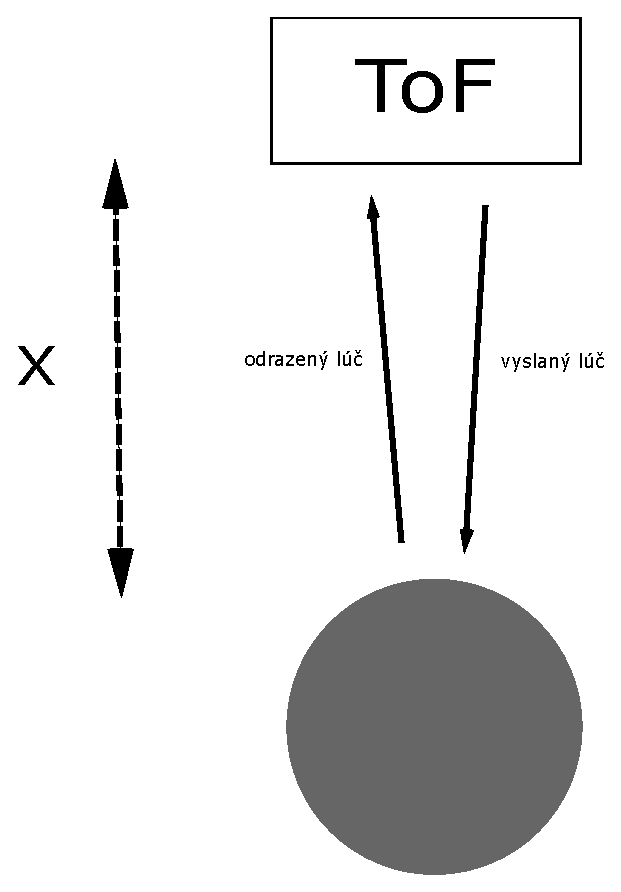
\includegraphics[width=60mm]{obr/ToF.eps}
	\caption{Princíp fungovania ToF senzora}\label{OBRAZOK 2.2.2} 
\end{figure} 

Hoci sme zvažovali aj iné typy snímačov vzdialenosti ako napríklad ultrazvukové alebo IR (infračervené) snímače, prišli sme k záveru, že najvhodnejším typom snímača bude práve ToF vďaka jeho malým rozmerom. Z možností ToF snímačov ponúkaných na trhu je pre naše zadanie VL6180X momentálne ideálnou možnosťou z dôvodu:
\begin{itemize}
	\item merateľného rozsahu - 100 mm
	\item presnosti merania - na 1 mm 
	\item malým rozmerom – 4.8 x 2.8 x 1.0 mm \cite{VL6180X}
\end{itemize}

Merateľný rozsah snímača je pre nás úplne postačujúci, keďže gulička sa pohybuje v trubičke práve o dĺžke 100 mm, s tým že v koncových bodoch sa nachádzajú ešte uzavretia trubičky, takže rozsah pohybu guličky je približne 90 mm, čo nám dáva ešte určitú rezervu. Dokonca veľa snímačov nespĺňa naše požiadavky práve z dôvodu že ich merateľný rozsah nezačína v 0 mm ale až pri vyšších hodnotách. Hoci presnosť meranie na 1 mm nie je pre riadenie systému ideálna, z ponúkaných senzorov sa nám nepodarilo v danej kategórii nájsť žiadny s lepšou presnosťou. Rozmery sú pre nás dôležité z hľadiska potreby umiestnenia snímača do jednej z koncových polôh trubičky aby sme mohli merať pozíciu guličky. Taktiež príliš veľké rozmery ako napríklad pri ultrazvukovom snímači by pre minimálne rozmery nášho zariadenia neboli vhodné z hladiska estetickosti. Vďaka minimálnym rozmerom snímača sa nám oproti pôvodnej verzii podarilo zmenšiť diel upevnenia snímača na trubičke, čím sme zlepšili aj estetickú zložku zariadenia.

\begin{figure}[]
	\centering
	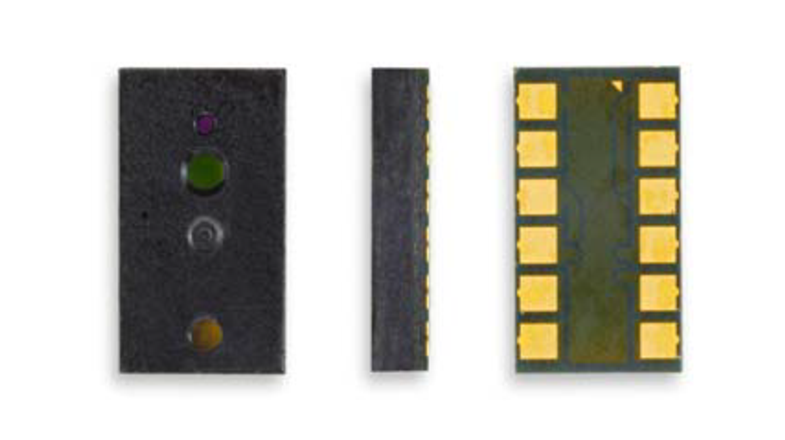
\includegraphics[width=60mm]{obr/VL6180X.eps}
	\caption{ToF snímač - VL6180X\cite{VL6180X}}\label{OBRAZOK 2.2.3} 
\end{figure} 
Na obrázku \ref{OBRAZOK 2.2.4} môžeme vidieť schému zapojenia snímača uvedenú v datasheete. V našej aplikácii sme piny 1 a 4 (GPI01 a GPIO0) nepoužívali a nechali sme ich voľné. Piny 5 a 6 – SCL a SDA, slúžiace na I2C komunikáciu snímača s mikropočítačom sú pomocou pull up rezistorov pripojené k napätiu. Za hodnoty pull up rezistorov sme zvolili odpor 10 kΩ. Ako môžeme vidieť v schéme piny 9 a 12 sú uzemnené a piny 10 a 8 sú zase pripojené k napájaniu, pričom sú k nim paralelne pripojené 2 kapacitory, ktorých hodnota je uvedená pre daný snímač v datasheete. Taktiež je spomenuté aby ich pozícia bola čo možno najbližšia k daným pinom.   
\begin{figure}[]
	\centering
	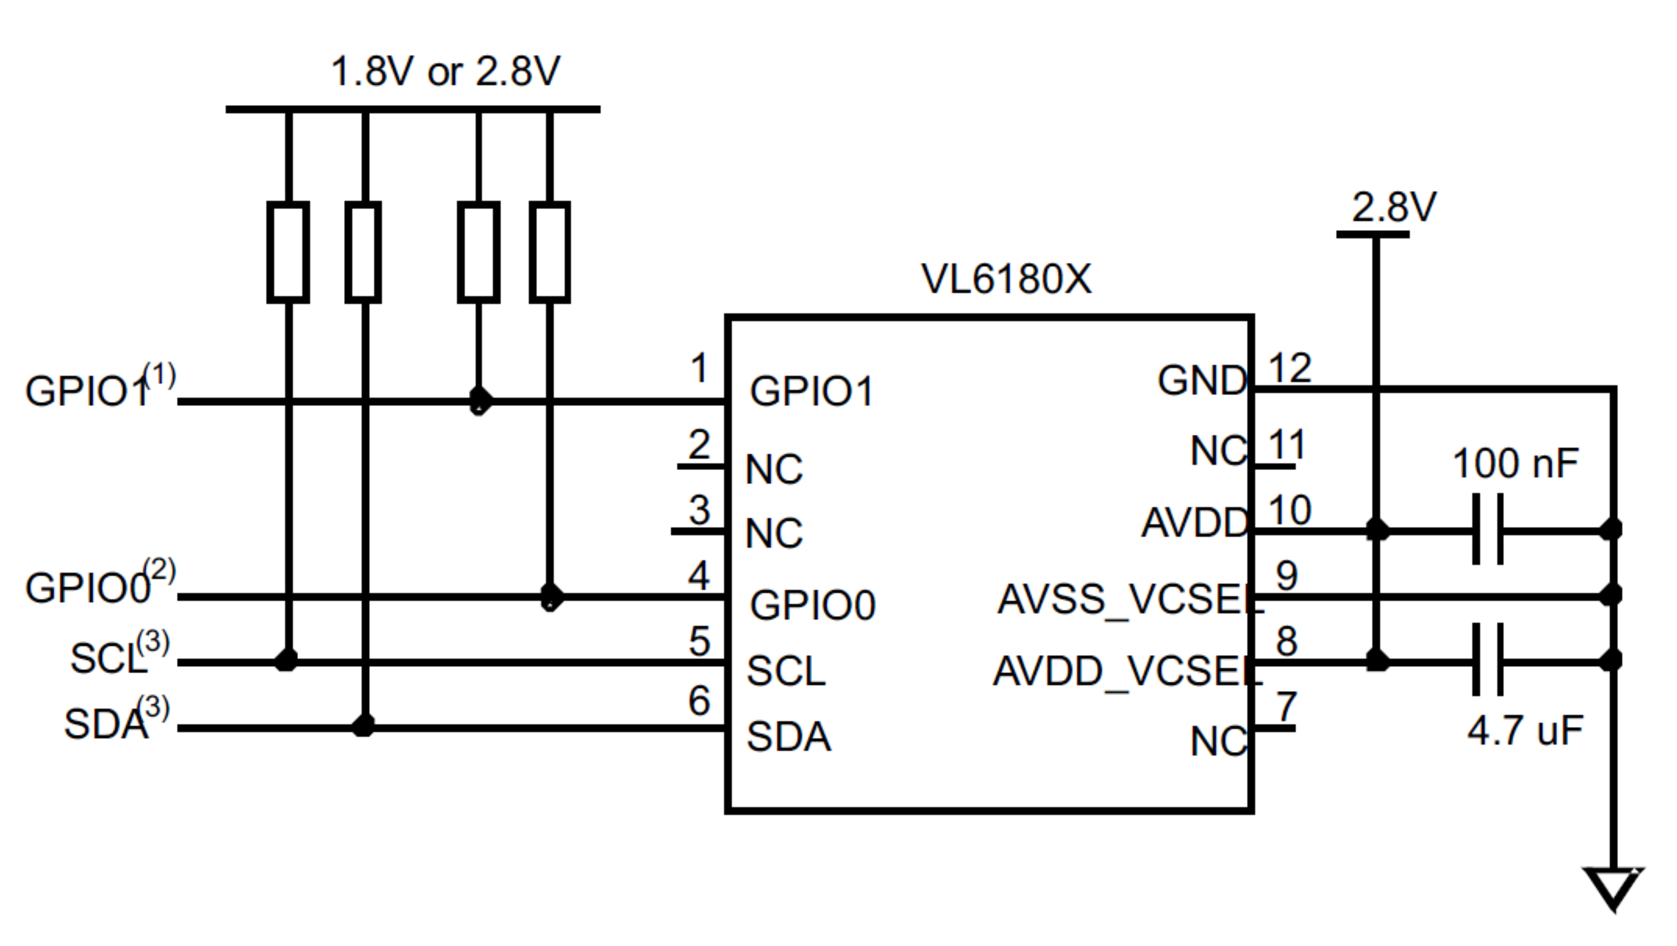
\includegraphics[width=130mm]{obr/VL6180Xscheme.eps}
	\caption{Schéma zapojenia snímača \cite{VL6180X}}\label{OBRAZOK 2.2.4} 
\end{figure} 

\subsection{Gyroskop - MPU 6050}
\label{kap:2.2.3}

Snímač MPU 6050 (obr. \ref{OBRAZOK 2.2.3.1}) je oproti pôvodným verziám zariadenia úplnou novinkou. Ide o 6 osový snímač pohybu – 3 osový gyroskop a 3 osový akcelerometer zostavený v malom balený o rozmeroch 4 x 4 x 0,9 mm. Jeho využitie je veľmi široké a stretnúť sa s ním môžeme pri smartfónoch alebo tabletoch. Poskytuje funkcie využívané pri aplikáciách ako navigácia, rozšírená realita, monitorovanie zdravia a pohybu a mnoho ďalších. Snímač užívateľovi poskytuje možnosť nastavenia meraného rozsahu v závislosti od aplikácie, pre ktorú bude využitý, teda pre sledovanie jednak rýchlych aj pomalých pohybov. Pri gyroskope si užívateľ môže vybrať z nasledujúcich rozsahov - ±250, ±500, ±1000 a ±2000\textdegree /s. U akcelerometra ide o rozsahy ±2g, ±4g, ±8g a ±16g.  Komunikácia s arduinom prebieha rovnako ako pri ToF snímači prostredníctvom I2C protokolu a rozsah napájacieho napätia 2,375V – 3,46 V \cite{MPU6050}.  

Jeho úlohou je merať uhol natočenia trubičky, na základe čoho vieme nastaviť trubičku do vodorovnej polohy.  

\begin{figure}[]
	\centering
	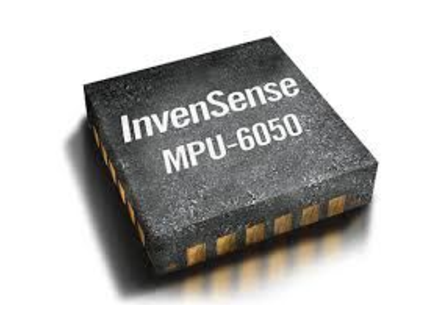
\includegraphics[width=60mm]{obr/MPU6050.eps}
	\caption{Schéma zapojenia snímača}\label{OBRAZOK 2.2.3.1} 
\end{figure} 


\subsection{Lineárny regulátor napätia - LDO}
\label{kap:2.2.4}

Z dôvodu tvorby vlastného braekoutu, na ktorom sú umiestnené oba naše snímače bolo potrebné nájsť vhodné napájacie napätie aby vyhovovalo obom snímačom a spadalo do ich rozsahov napätí. Pre snímač VL6180X je vstupné napätia v rozmedzí 2,6 V - 3,0 V \cite{VL6180X} a pri MPU6050 ide o rozsah 2,375 – 3,46 V\cite{MPU6050}. Arduino nám ponúka len 2 úrovne napájania a to 3,3 V a 5 V. Ak by sme využívali len snímač MPU6050 mohli by sme priamo využiť napájanie 3,3 V, ktoré spadá do jeho pracovného rozsahu, no pre snímač polohy je táto možnosť nevyhovujúca. Preto je potrebné upraviť ponúkané úrovne napätia z arduino dosky do rozsahu 2,6 - 3,0 V, vyhovujúcemu obom snímačom. O zmenu napätia sa stará lineárny regulátor napätia – STM732M28R od firmy STMicroelectronics , ktorý vstupné napätie v rozsahu 2,5 – 28 V prevádza na úroveň 2,8 V. Táto hladina je vyhovujúca pre oba snímače.   

\begin{figure}[]
	\centering
	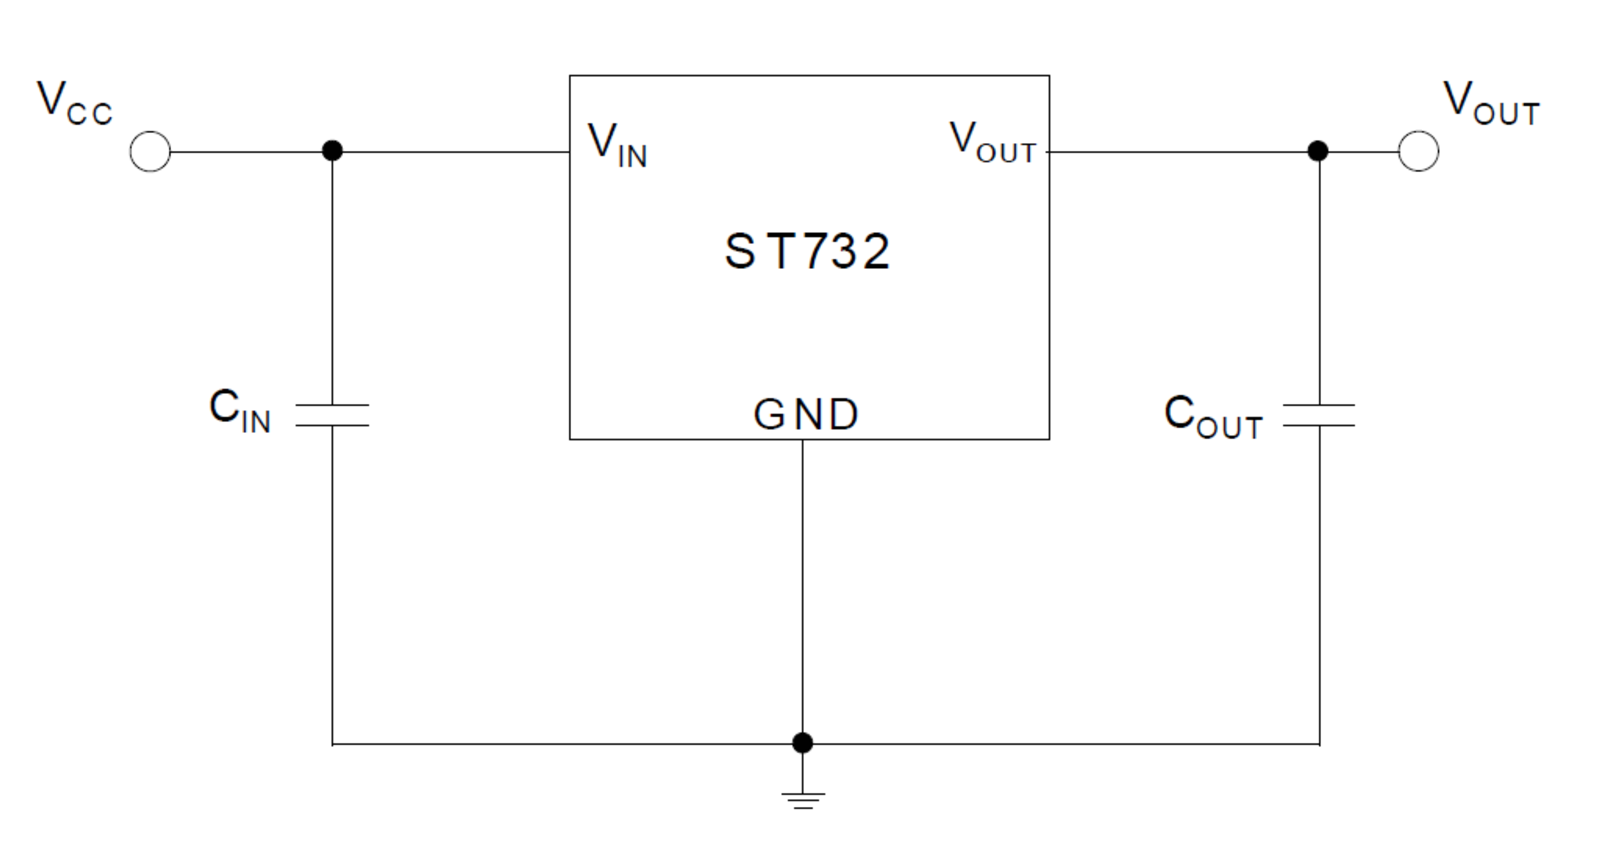
\includegraphics[width=100mm]{obr/LDOscheme.eps}
	\caption{Schéma zapojenia snímača\cite{LDO}}\label{OBRAZOK 2.2.4.1} 
\end{figure} 

\section{Teleso}
\label{kap:2.3}

Dôležitou časťou celého systému je práve gulička, pohybujúca sa v trubičke, ktorej polohu sledujeme a riadime. Na náš systém vplýva ako jej hmotnosť a tvar tak aj kvalita a farba jej povrchu. Keďže na meranie polohy guličky používame ToF snímač, ktorý meria vzdialenosť na základe času, za ktorý sa svetelný lúč vyslaný zo senzora odrazí od telesa a vráti naspäť, na kvalitu merania vplývajú aj tieto parametre. 

Výrobca v datasheete \cite{VL6180X} uvádza nezávislosť merania od farby alebo kvality povrchu telesa. Deklarované je to aj grafom na obrázku \ref{OBRAZOK 2.3.1} , kde môžeme vidieť, že hodnoty pre telesá rozdielnej odrazivosti sa navzájom nelíšia a nachádzajú sa v tom istom rozsahu.

Aj napriek tomu sme v našich meraniach sme mohli sledovať odlišnosti v presnosti pre rôzne typy guľôčok. 
\begin{figure}[]
	\centering
	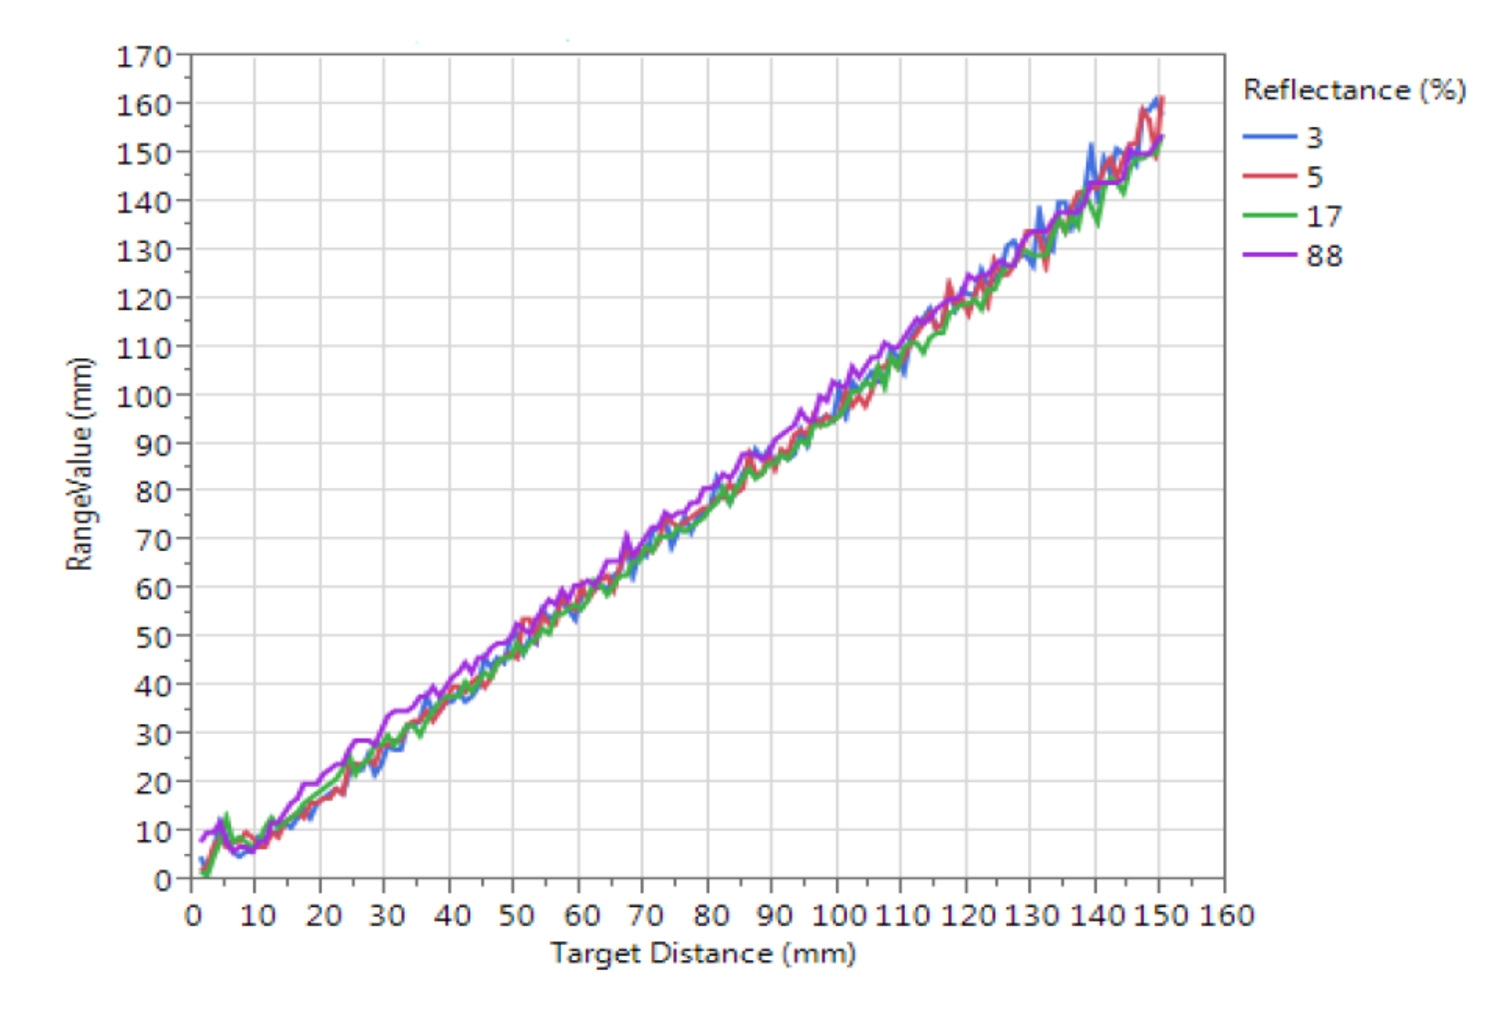
\includegraphics[width=100mm]{obr/TOFreflectance.eps}
	\caption{Závislosť merania od odrazivosti telesa\cite{VL6180X}}\label{OBRAZOK 2.3.1} 
\end{figure} 
Tento fakt môže byť ovplyvnený práve tvarom meraného telesa, ktorý pre funkčnosť snímača nie je ideálny, no pre potreby nášho zadania nevyhnutný. Svetelný lúč nedopadá na kolmý povrch, preto nemusí byť odrazený práve pod takým uhlom aby ho dokázal snímač adekvátne zachytiť a zanalyzovať. Na základe tohto faktu sme predpokladali, že by ideálnym riešením bolo teleso s povrchom, ktorý čo najviac rozptýli dopadajúci lúč aby šanca, že sa lúč od neho odrazí k snímaču bola čo najvyššia, čím by sa zlepšila kvalita merania. Ďalšou požiadavkou pri hľadaní ideálneho telesa bola dostatočná hmotnosť guličky aby na zmenu stavu systému reagovala v reakčnom čase dostatočne dlhom aby náš riadiaci systém stíhal vykonávať potrebné výpočty, no zároveň nechceme aby bol zbytočne dlhý. Na túto požiadavku vplýva aj kvalita povrchu guličky. Aby sa gulička mohla voľne pohybovať v trubičke, nič jej nebránilo a tak nevplývalo na systém je potrebné aby bol jej tvar čo najviac podobný tvaru ideálnej gule. Poslednou požiadavkou bola jeho jednoduchá dostupnosť. Keďže sa jedná o open source projekt, je potrebné aby sa každý, kto by mal záujem o zostrojenie nášho zariadenia vedel ku danej guličke bez väčších problémov dostať. 

Z možností dostupných na trhu sme sa rozhodli otestovať náš snímač  pre viacero typov materiálov: 
 drevo, silikón, POM - polyoxymetylén, NBR - butadien-akrilonitrilový kaučuk (syntetická guma), NR - prírodná guma, oceľ a PP - polypropylén.


Pri meraní sme postupovali nasledovne. Guličku sme nastavili do krajnej polohy v trubičke (vzdialenosť 90 mm), následne sme pomocou ToF snímača zmerali 100 hodnôt jej aktuálnej polohy. Hodnoty sme vložili do tabuľky a pomocou vzorca \ref{rovnica.2.3.1} sme vypočítali smerodajnú odchýlku pre dané meranie.
\begin{align}
	\label{rovnica.2.3.1}
	\sigma = \sqrt{\frac{1}{N}\sum_{i=1}^{N}(x_i-\bar{x})^{2}}
\end{align} Tento postup sme zopakovali pre všetky materiály. V tabuľke \ref{TABULKA_2_1} môžeme vidieť porovnanie smerodajných odchýlok pre jednotlivé materiály. Na základe merania, ktoré sme vykonali, môžeme tvrdiť, že náš snímač dosahuje najmenšie smerodajné odchýlky pri materiály PP – polypropylén a najväčšie odchýlky pri NBR – syntetická guma. 


\begin{table}[ht]
	\centering
    \begin{tabular}{|l|l|l|l|l|l|l|l|}
    	\hline
    	\textbf{Materiál}            & silikón & POM    & drevo  & NBR                            & NR     & oceľ & PP                             \\ \hline
    	\textbf{smerodajná odchýlka} & 1,27    & 1,2891 & 1,3644 & \cellcolor[HTML]{FFCCC9}1,6271 & 1,3322 & 1,5  & \cellcolor[HTML]{9AFF99}1,2595 \\ \hline
    \end{tabular}
	
    \caption{Smerodajné odchýlky pre dané materiály}
    \label{TABULKA_2_1}
\end{table}
Ako bolo vyššie spomenuté, dynamika systému má veľký vplyv na jeho riadenie. Z toho dôvodu je pri výbere guličky dôležitá práve rýchlosť akou sa gulička v systéme pohybuje. Ak je gulička príliš rýchla  , riadiaci systém má menej času reagovať na zmenu jej polohy, ktorá sa hlavne pri výraznej zmene referenčnej hodnoty výrazne mení. Keďže dĺžka trubičky je pomerne malá (100 mm), ak riadiaci systém nedokáže včas zareagovať  na zmenu jej polohy bude dochádzať k nárazom guličky do krajných polôh trubičky, čo je pri riadení nežiaduci jav. Z toho dôvodu sa snažíme voliť guličku, ktorej rýchlosť je adekvátna pre našu aplikáciu. Rýchlosť guličky je závislá jednak od jej hmotnosti, materiálu, kvality povrchu a rozmerov.
Pri meraní sme zaznamenávali polohu guličky a čas, v ktorom sa v danej polohe nachádzala. Pohyb guličky bol z jednej krajnej polohy trubičky do druhej krajnej polohy pri naklonení trubičky o uhol 5 \degree. Následne sme namerané hodnoty vykreslili do grafu v programe MATLAB a pomocou analýzy grafu sme našli čas, za ktorý gulička prešla danú vzdialenosť trubičky. Hodnoty sme zapísali do tabuľky a vypočítali rýchlosť jednotlivých guličiek.

\begin{table}[ht]
	\centering
	\begin{tabular}{|l|l|l|l|l|l|l|l|}
		\hline
		\textbf{Materiál}           & silikón & POM    & drevo  & NBR                            & NR     & oceľ                           & PP                             \\ \hline
		\textbf{rýchlosť {[}m/s{]}} & 0,0862  & 0,1035 & 0,1178 & \cellcolor[HTML]{9AFF99}0,0766 & 0,1128 & \cellcolor[HTML]{FFCCC9}0,1214 & \cellcolor[HTML]{FFFFFF}0,0895 \\ \hline
	\end{tabular}
    \caption{Rýchlosti guličiek pre dané materiály}
    \label{TABULKA_2_2}
\end{table}

V tabuľke \ref{TABULKA_2_2} môžeme vidieť porovnanie rýchlosti jednotlivých guličiek pri pohybe mierne naklonenou trubičkou. Najpomalšie sa pohybujúcou je gulička z NBR, ktorá oproti guličke z ocele, použitej v pôvodných verziách zariadenia dosahuje takmer polovičné priemerné rýchlosti.  
Na základe vykonaných meraní sme sa rozhodli zvoliť si za teleso v systéme guličku vyrobenú z polypropylénu (PP). Snímač dosahuje pri danej guličke najpresnejšie merania, takže meraná poloha guličky sa najviac približuje jej skutočnej polohe. Meranie s čo najmenšou smerodajnou odchylkou je pri riadení systému kľúčové, no treba uvažovať aj dynamiku guličky. Z nameraných rýchlostí guličiek by pre nás bola najvhodnejšou voľbou gulička z NBR, no jej presnosti merania sú výrazne horšie v porovnaní s guličkou PP. Tá ale dosahuje tiež prijateľné rýchlosti pre našu aplikáciu, preto sme si ju vybrali za naše teleso z nami testovaných guličiek.

Ak porovnáme guličku z ocele, ktorá je telesom použitým v pôvodnej verzii a guličky z PP, ktorú sme na základe meraní vybrali, môžeme pozorovať výrazné zlepšenie merania snímača z hľadiska smerodajných odchýlok ako aj spomalenie pohybu guličky v trubičke. 

\section{Prevod rotačného pohybu - servo, trubička}  
\label{kap:2.4}

Aktuátorom v našom zariadení je servo motor, no aby mohol vytvárať akčný zásah (pootočenie trubičky) do systému, ktorým je naša trubičke s guličkou, musí prísť ku prenosu rotačnému pohybu.
 
V pôvodnej verzii zariadenia bol tento prevod riešený priamym upevnením trubičky na Servo motor, čo znamená, že otočenie trubičky sa rovnalo otočeniu serva o príslušný uhol z rozsahu ±30\textdegree, ktorý bol stanovený. Najmenší možný uhol pootočenia trubičky sa teda rovnal presnosti serva : 1\textdegree. Vzhľadom na malé rozmery trubičky ide o pomerne veľký uhol. Malé možné rozlíšenie uhlu, o ktorý vieme otočiť trubičku so sebou prináša obmedzenia pri riadení systému, kedy akčný zásah nemôže nadobúdať takú množinu hodnôt. To má za následok neschopnosť nastaviť tak presný akčný zásah aby sa čo najviac približoval hodnote vypočítanej riadiacim systémom. 

Našim riešením tohto problému je použitie jednoduchého prevodu, cez ktorý budeme prenášať rotačný pohyb serva na trubičky. Prevod sa skladá z 2 koliesok rozdielnych priemerov, pričom jedno je upevnené na servo motor a k druhému je pripevnená trubička. Prenos pohybu z jedného kolieska na druhé je riešené pomocou ozubeného remeňa GT2 o šírke 6 mm, bežne používanom pri krokových motoroch alebo 3D tlačiarňach. Výhodou nášho riešenia je využitie takmer celého rozsahu pohybu nášho servo motora. Kým pri pôvodnom zariadení išlo o využitie rozsahu ±30\textdegree z možných ±90\textdegree,  v danom riešení využívame rozsah ±75\textdegree.

Prevodový pomer - $p$ a následne aj rozmery koliesok ($d1$ - vstupný priemer, $d2$ - výstupný priemer) sme vypočítali na základe vzorcov (\ref{rovnica.2.4.1}) pre výpočet prevodov, kde najprv zistíme prevodový pomer na základe vstupného a výstupného rozsahu otočenia. Vzorce sa dajú jednoducho odvodiť na základe dĺžky posunutia remeňa - x, ktorá je na oboch kolieskach vždy rovnaká. Ide o dĺžku kružnicového oblúka, o priemere daného kolieska, ktorého uhol je rovný uhlu otočenia (obr.\ref{OBRAZOK 2.4.1}). Tento uhol môžeme pri výpočtoch nahradiť rozsahom otáčania jednotlivých koliesok.  Za výstupný rozsah sme si zvolili ±15\textdegree, pre dĺžku trubičky je tento uhol postačujúci keďže referenčná hodnota sa pohybuje od 0 po 100 mm a gulička sa pohybuje v trubičke dostatočne veľkou rýchlosťou bez väčšieho odporu, nemusí dochádzať k tak výrazným zásahom aktuátora ako je naklonenie o celých 30\textdegree, či už kladným alebo záporným smerom.  Reakcia systému je aj pri nami zvolenom rozsahu dostatočne rýchla. Pre vstupný rozsah sme si zadali ±75\textdegree aby sme disponovali určitou rezervou voči maximálnemu rozsahu otočenia.



\begin{align}
	\label{rovnica.2.4.1}
	p &= \frac{d1}{d2} \\
	x_1&=\frac{\pi*d_1*\alpha_1}{360} \\
	x_2&=\frac{\pi*d_2*\alpha_2}{360}
\end{align}

\begin{figure}[!h]
	\centering
	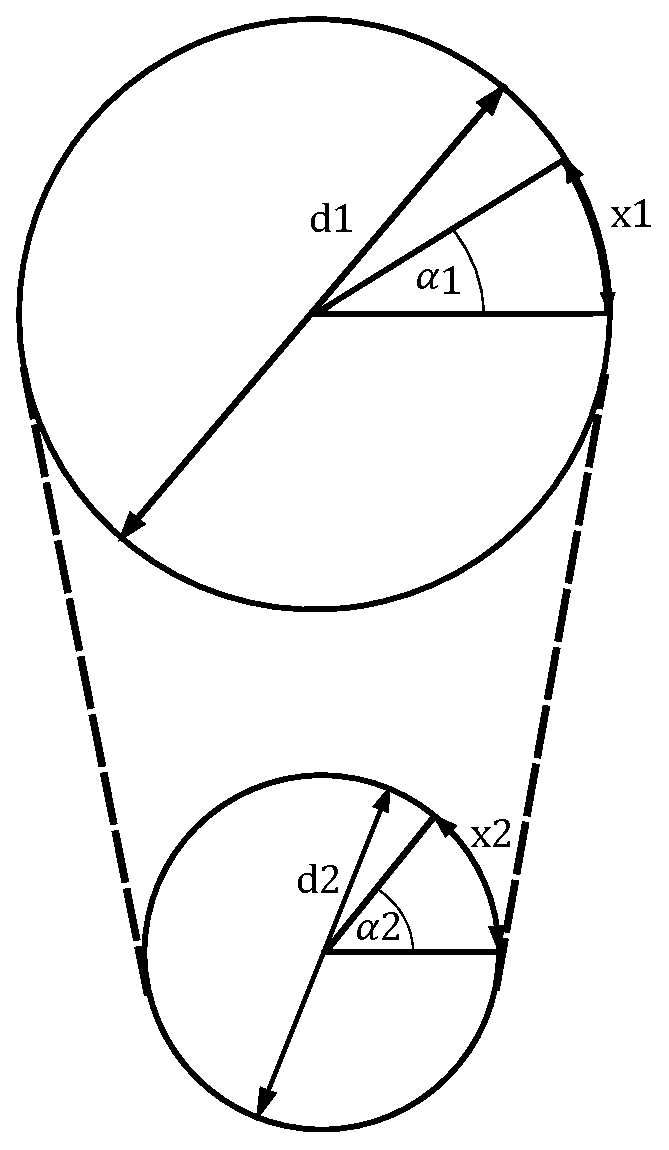
\includegraphics[width=50mm]{obr/prevod.eps}
	\caption{Posunutie remeňa pri rotácii kolieska}\label{OBRAZOK 2.4.1} 
\end{figure} 

\begin{align}
	\label{rovnica.2.4.2}
		x_1 &= x_2 \\
	p &=\frac{d_1}{d_2}=\frac{\alpha_1}{\alpha_2} \\
	p &=\frac{30\degree}{150\degree}=0.2
\end{align}
Na základe prevodového pomeru vieme povedať, že na 1\textdegree otočenia serva prislúcha 0,2\textdegree otočenia trubičky. Týmto prevodom sme teda 5 násobne zväčšili množinu hodnôt, ktoré môže aktuátor nadobudnúť a tým zvýšili presnosť akčného zásahu do systému. 
Ak poznáme prevodový pomer rozmery koliesok získame voľbou priemeru jedného z nich a následným výpočtom priemeru druhého kolieska na základe vzorca \ref{rovnica.2.4.1}. Za priemer kolieska pripojeného k servo motoru sme si zvolili $d1 = 10 mm$. Je to dostatočná veľkosť pre uchytenie kolieska a prevod pohybu pomocou remeňa, no zároveň šetríme miesto aby sme zachovali minimálne rozmery pôvodnej verzie zariadenia. Z toho vyplýva, že priemer druhého kolieska bude $d2 = 50 mm$.  





\section{3D prvky}
\label{kap:2.5}


Z dôvodu zmeny hardvéru ako je napríklad vytvorenie vlastnej PCB dosky pre snímače, došlo  k potrebe návrhu nového 3D modelu zariadenia a aktualizácii jeho starších prvkov.  Najvýraznejšou zmenou je použitie prevodu (kap. \ref{kap:2.4}) na prenos rotačného pohybu zo serva na trubičku. Pre implementáciu tohto prevodu bolo potrebné vytvoriť hneď niekoľko nových 3D prvkov a niektoré staršie prešli menšími zmenami. Tiež sme pri ich návrhu museli hľadieť na viacero požiadaviek kladených na tento prevodový systém, ako je potreba možnosti napínania remeňa alebo jeho upevnenie na prevodovom koliesku. Na obrázku \ref{OBRAZOK 2.5.1} môžeme vidieť už výslednú formu 3D modelu zariadenia, ktorá sa skladá z niekoľkých samostatných prvkov, ktorých funkcie si vysvetlíme v tejto sekcii. Všetky prvky boli navrhnuté v CAD programe Fusion 360.
\begin{figure}[!h]
	\centering
	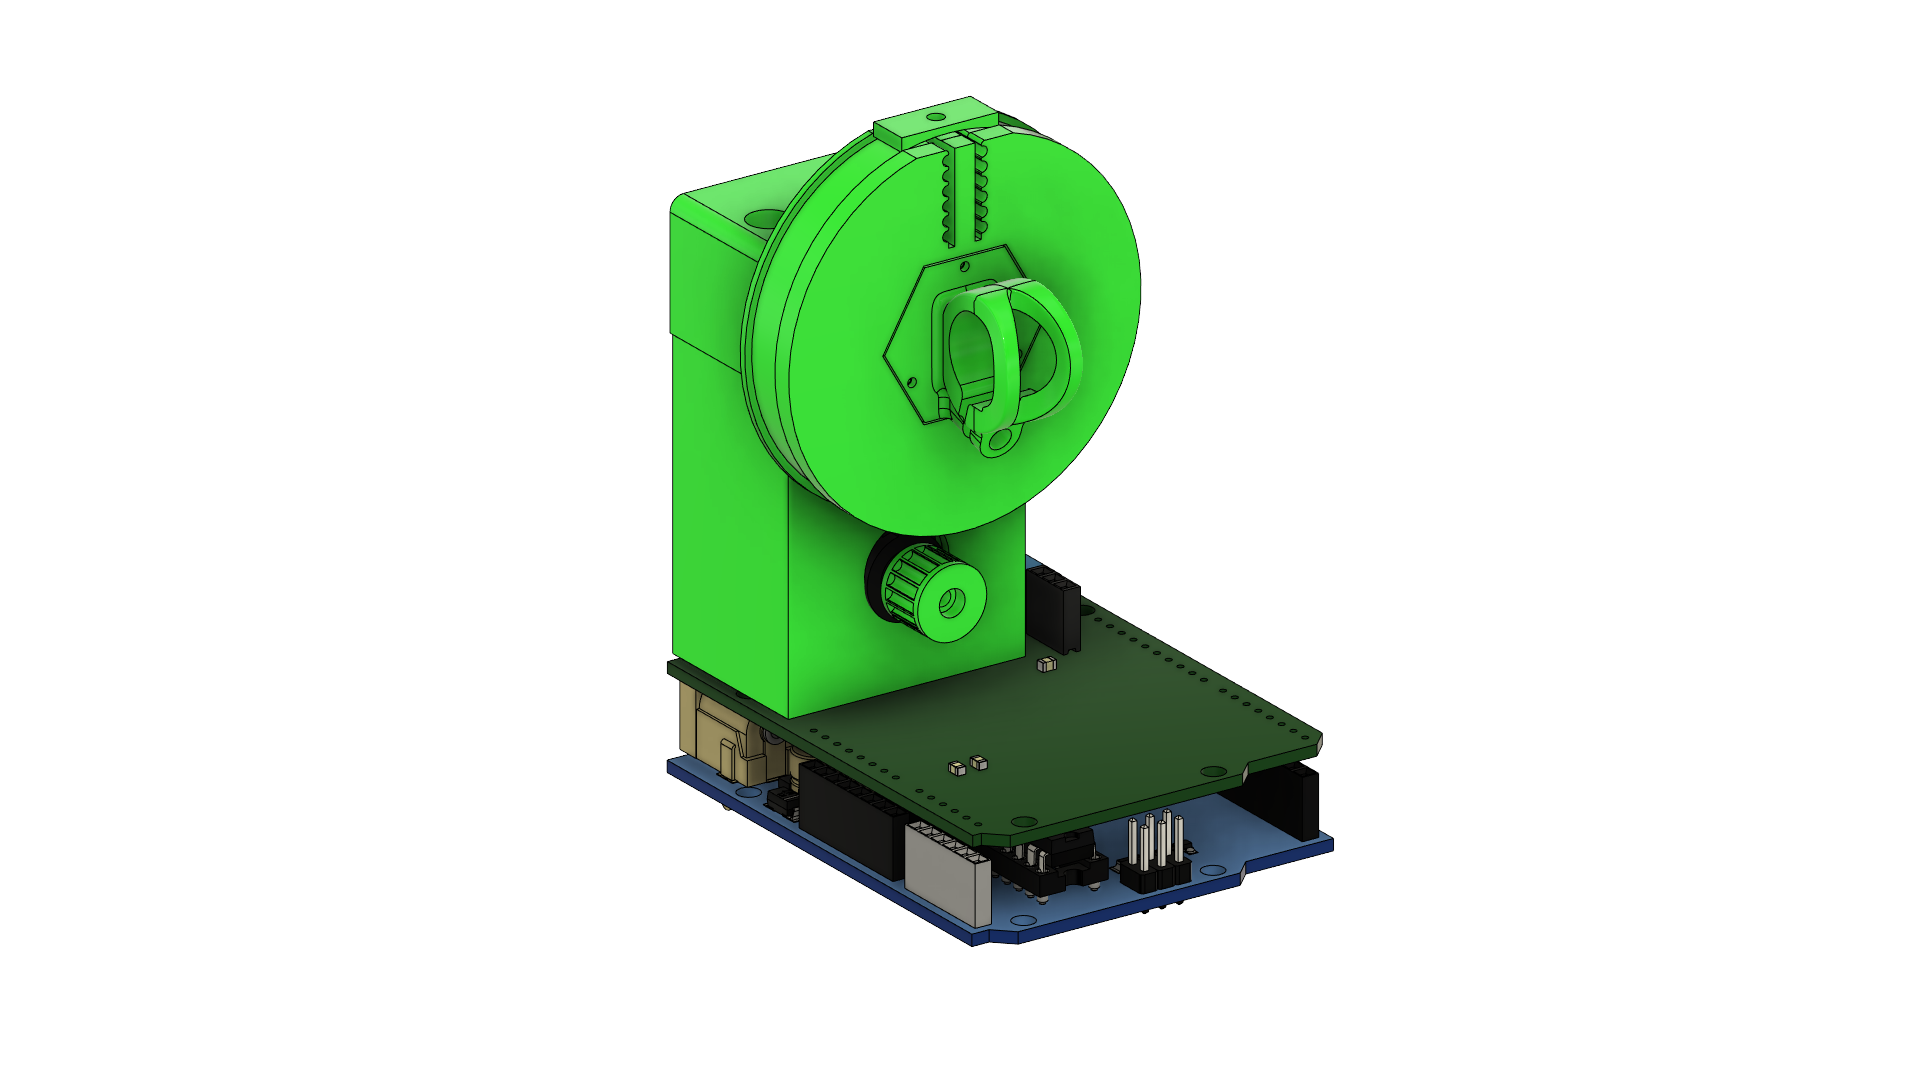
\includegraphics[width=150mm]{obr/3Dmodel.png}
	\caption{3D model zariadenia }\label{OBRAZOK 2.5.1} 
\end{figure} 

Prvým prvkom je diel uložený priamo na PCB doske, ktorý slúži na uloženie servo motora. Môžeme ho vidieť na obrázku \ref{OBRAZOK 2.5.2} a) prvok.  Pri umiestnení servo motora v danom diely sme sa snažili aby sa poloha hriadeľa nachádzala v čo možno najnižšej polohe aby sme tak šetrili miesto a minimalizovali rozmery zariadenia. Pripevnenie k prvku je prevedené pomocou závrtných skrutiek. Tiež sme sa rozhodli o schovanie servo motora do vnútra prvku a jeho vkladanie cez zadnú stranu, čím jednak šetríme priestor no zároveň pri montáži nedochádza k problému s káblami servo motora, ktoré majú dostatočne veľa priestoru a nemalo by dôjsť k ich poškodeniu.  Okrem toho sa v prvku nachádza drážka, v ktorá slúži na vedenie druhého dielu pri vykonávaní translačného pohybu smerom nahor a nadol, čím je splnená funkcia napínania remeňa.  Taktiež slúži na pripojenie celého modelu k PCB doske pomocou 2 skrutiek.

Druhým prvkom (obr. \ref{OBRAZOK 2.5.2}, prvok b) je už spomenutý diel, ktorý sa zasúva do prvého dielu.  Translačný pohyb je zabezpečený 2 skrutkami M3 o dĺžke 20 mm, ktoré sa zapierajú o spodný diel a tým zabezpečujú zdvih celého dielu. Výška zdvihu sa nastavuje zaskrutkovávaním skrutiek do samoistiacich matíc, ktoré sú schované v samotnom telese (obr. \ref{OBRAZOK 2.5.3}). Ich uloženie sme vykonali zastaveným tlače v danej vrstve, v ktorej sa v telese nachádzajú a po vložení matíc bola tlač znova obnovená.  Aby nedochádzalo k postupnému uvoľňovaniu spoja pri prevádzke zariadenia, čo by malo za následok uvoľnenie napätia v remeni, rozhodli sme sa pre voľbu samotesniacich matíc. Sila, ktorou je teleso ťahané smerom dole je vyvolaná tlakom remeňa na prevodové koliesko, ktoré je pomocou skrutky M5 uchytené na tomto prvku. V zadnej časti môžeme vidieť výrez na umiestnenie matice pre daný skrutkový spoj. Teda okrem napínania remeňa je jeho úlohou taktiež uchytenie veľkého prevodového kolieska. Na obrázku \ref{OBRAZOK 2.5.2} môžeme tiež vidieť uloženie druhého dielu v prvom diele z prednej a) a zadnej b) strany.  

\begin{figure}[]
	\centering
	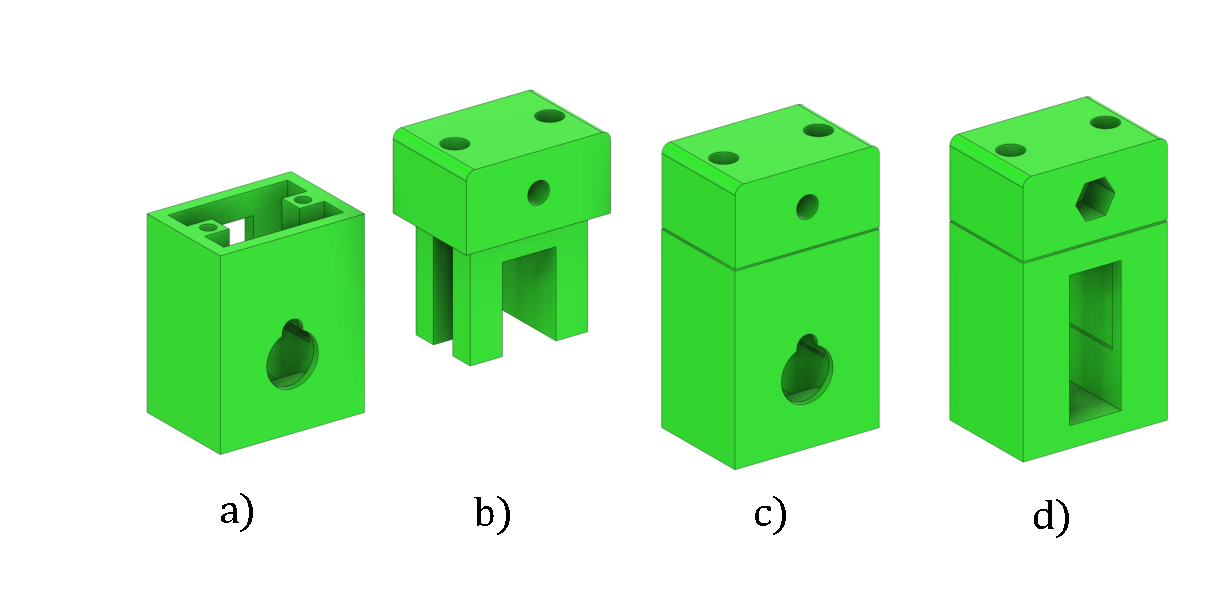
\includegraphics[width=150mm]{obr/3Dbase.eps}
	\caption{Uloženie prvého a druhého dielu}\label{OBRAZOK 2.5.2} 
\end{figure} 

\begin{figure}[]
	\centering
	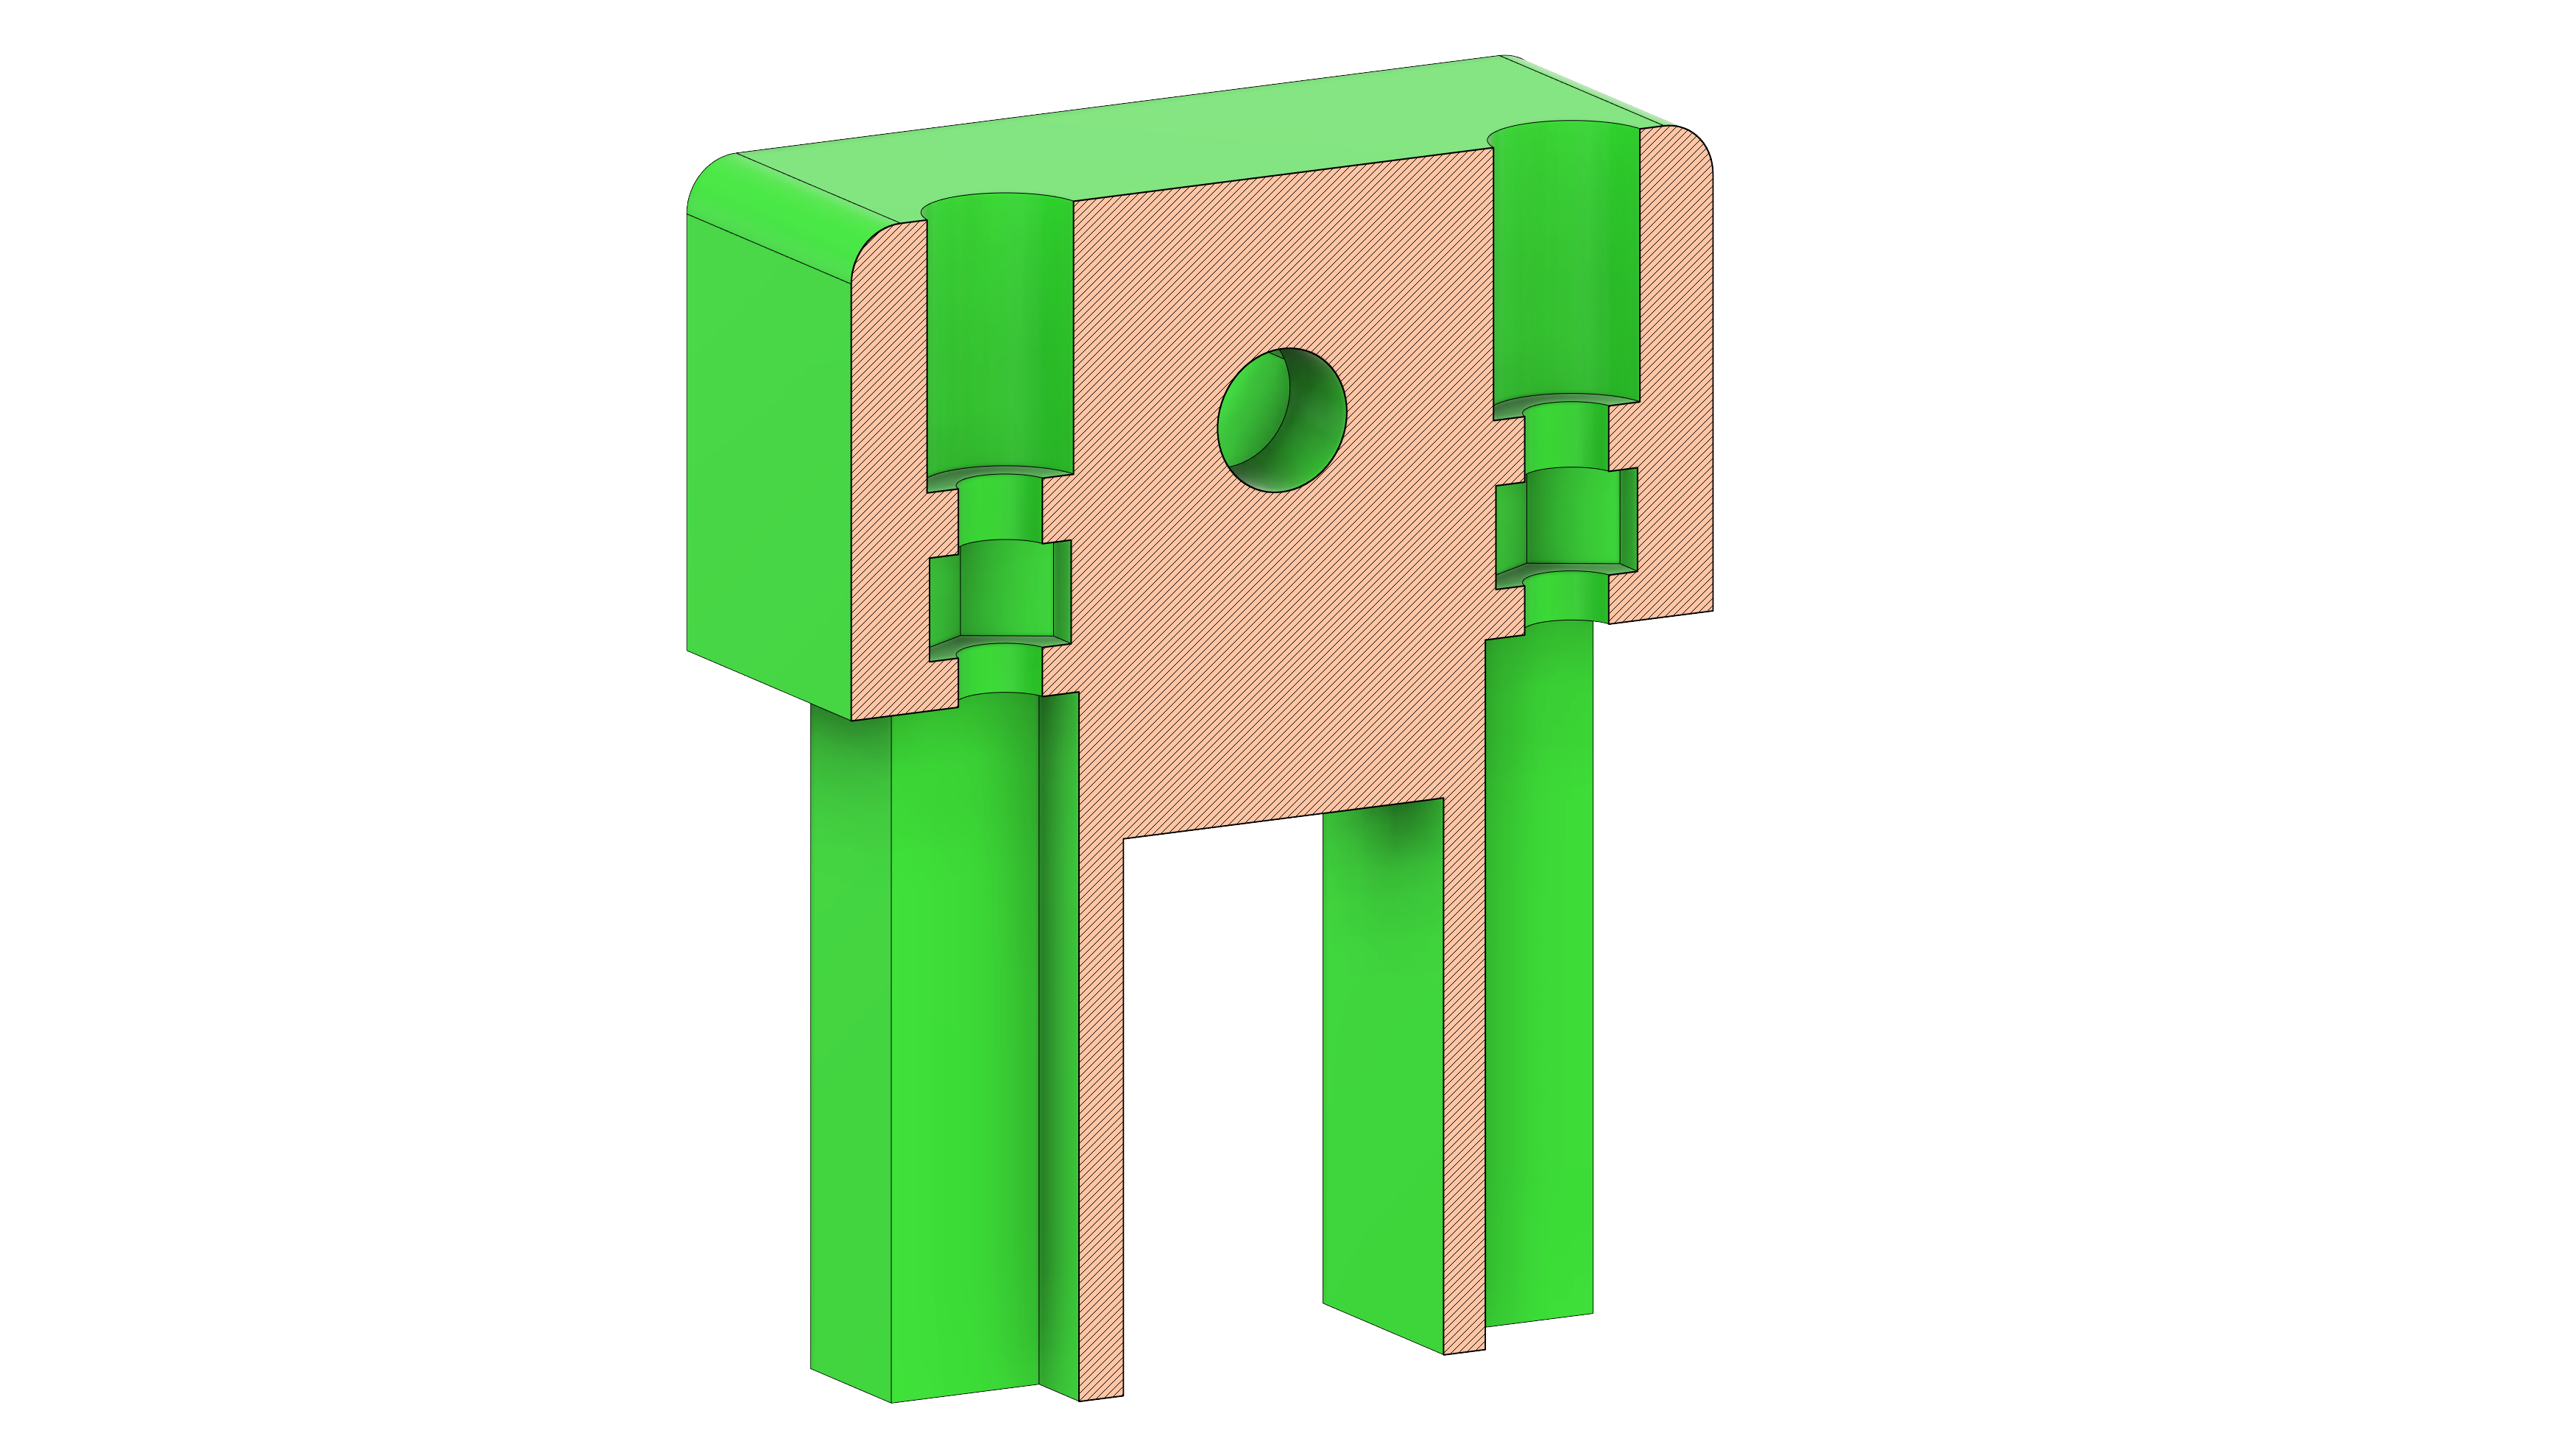
\includegraphics[width=70mm]{obr/3Dprvok2.png}
	\caption{Uloženie poistných matíc}\label{OBRAZOK 2.5.3} 
\end{figure} 

Ďalším prvkom je uchytenie trubičky na prevodové koliesko (obr. \ref{OBRAZOK 2.5.4}, prvok a). Ide o aktualizáciu a miernu úpravu pôvodnej verzie tohto prvku, ktorú môžeme vidieť na obrázku \ref{OBRAZOK 2.5.4} ako prvok b). Keďže pôvodne sa zachytával priamo na hriadeľ servo motora, zmenou prešla práve časť uchytenia prvku. Pripevnenie držiaka ku koliesku sme sa rozhodli riešiť pomocou 3 samorezných skrutiek. Pre zabezpečenie jeho presného uloženia, tvar držiaka sme navrhli tak aby pri montáži zapadol do kolieska, v ktorom sa nachádza výrez rovnakého tvaru. 

\begin{figure}[]
	\centering
	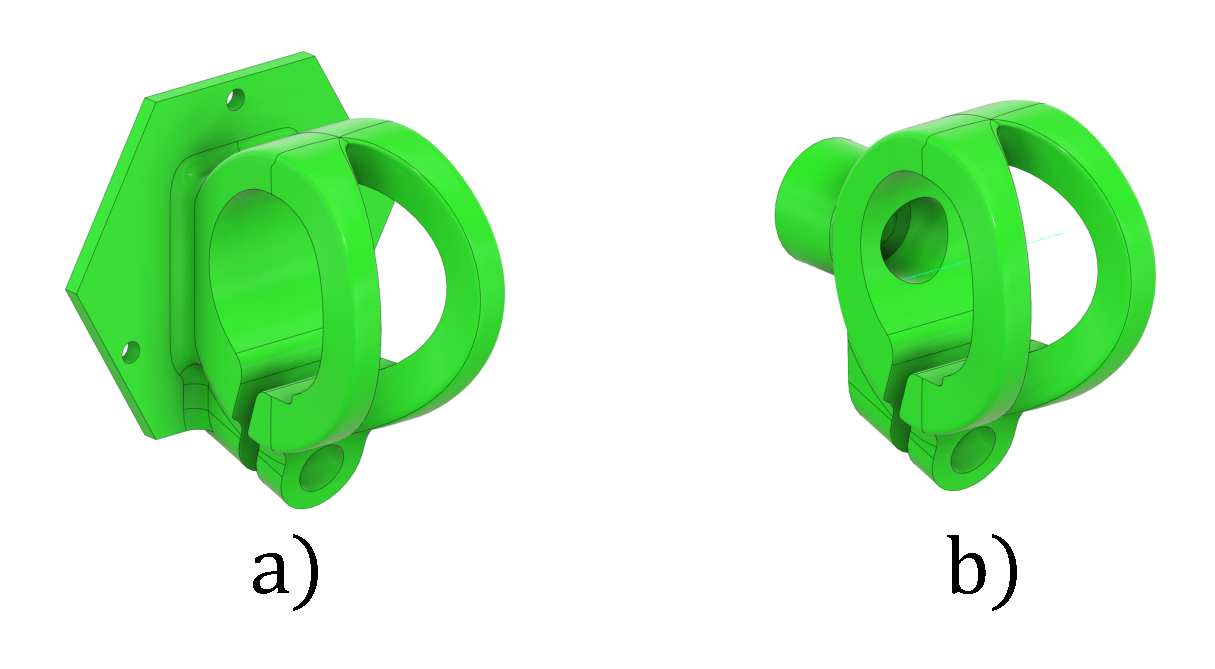
\includegraphics[width=70mm]{obr/3Ddrziak.eps}
	\caption{Uloženie poistných matíc}\label{OBRAZOK 2.5.4} 
\end{figure} 

Poslednými prvkami sú samotné prevodové kolieska, ktoré spĺňajú nami vypočítané parametre (prevodový pomer). Môžeme ich vidieť na obrázku \ref{OBRAZOK 2.5.5}. Na koliesku o priemere 10 mm sa nachádza po celom vonkajšom obvode ozubenie dimenzované pre náš remeň a pre upevnenie kolieska ku hriadeľu serva sme namodelovali vnútorné ozubenie, ktoré zodpovedá zúbkovaniu hriadeľa. Uchytenie k servo motoru po nasunutí kolieska na hriadeľ je prevedené pomocou skrutky M2. Koliesko o priemere 50 mm má po obvode drážku pre vedenie remeňa, ktorá bráni pred jeho vysunutím. Upevnenie remeňa na koliesko je zabezpečené pomocou výrezu v tvare profilu remeňa, a nachádza sa v hornej časti kolieska. Po nasunutí remeňa do výrezov je následne ešte poistený priskrutkovaním malej plôšky ku samotnému koliesku, ktorá na remeň pôsobí prítlačnou silou. Upevnenie kolieska na konštrukciu modelu je prevedené cez ložisko, aby sa mohlo koliesko voľne pohybovať pri otáčaní servo motora. Ložisko je uložené vo výreze v strede kolieska, kde sa zadnou stenou vonkajšieho krúžka opiera o koliesko a ku modelu je pripevnené skrutkou M5, ktorá sa zapiera o zadnú stranu jeho vnútorného krúžka.   
 
 \begin{figure}[]
 	\centering
 	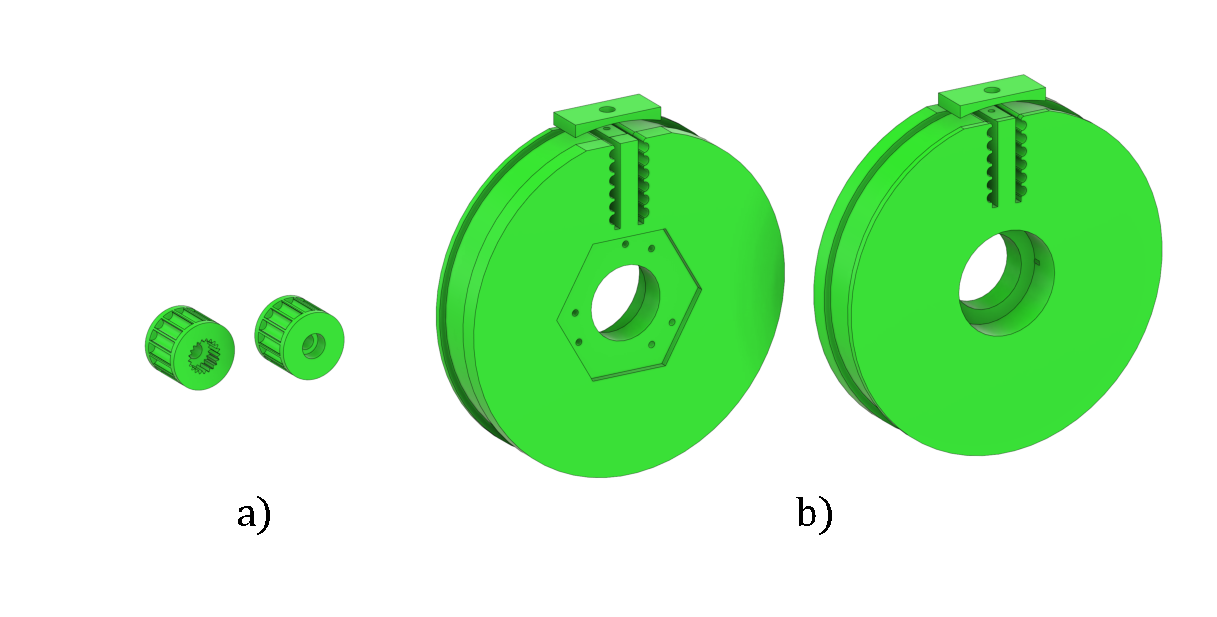
\includegraphics[width=150mm]{obr/3Dkolieska.eps}
 	\caption{Uloženie poistných matíc}\label{OBRAZOK 2.5.5} 
 \end{figure} 